% ============================================================
% IEEE Conference Paper — GenAI Assignment #1
% ============================================================
\documentclass[conference]{IEEEtran}

% ── Packages ────────────────────────────────────────────────
\usepackage{cite}
\usepackage{amsmath,amssymb,amsfonts}
\usepackage{algorithmic}
\usepackage{graphicx}
\usepackage{textcomp}
\usepackage{xcolor}
\usepackage{booktabs}
\usepackage{multirow}
\usepackage{subcaption}
\usepackage{hyperref}
\usepackage{float}
\usepackage{tabularx}
\usepackage{array}
\usepackage{tikz}
\usetikzlibrary{shapes.geometric, arrows, positioning, fit, calc}

\hypersetup{
  colorlinks=true,
  linkcolor=blue,
  citecolor=blue,
  urlcolor=blue
}

\graphicspath{{../results/}{../reports/figures/}}

\def\BibTeX{{\rm B\kern-.05em{\sc i\kern-.025em b}\kern-.08em
    T\kern-.1667em\lower.7ex\hbox{E}\kern-.125emX}}

\begin{document}

% ============================================================
\title{Multi-Corruption Image Restoration and Style-Conditioned Face-to-Sketch Generation: A Unified Framework with Autoencoder, Mixture-of-Experts, and Conditional GAN Architectures}

\author{
\IEEEauthorblockN{Fahad Bin Faisal}
\IEEEauthorblockA{
Roll Number: i230614\\
Generative AI — Assignment \#1\\
\textit{GitHub:} \url{https://github.com/fhd-fsl/GenAI-A1}
}
}

\maketitle

% ============================================================
\begin{abstract}
This paper presents the design, implementation, evaluation, and deployment of four generative AI systems for image restoration and synthesis. Tasks~1--3 address multi-corruption image restoration on the Oxford-IIIT Pet Dataset using progressively more sophisticated architectures: (1)~a universal denoising autoencoder with a strict information bottleneck, (2)~a corruption classifier with hard-routed specialist autoencoders, and (3)~a jointly trained soft mixture-of-experts model with temperature-scaled gating. Task~4 addresses style-conditioned face-to-sketch generation on the FS2K dataset using a conditional generative adversarial network with a U-Net generator and PatchGAN discriminator. All models are trained in PyTorch with Optuna hyperparameter optimization (20 trials per task) and experiment tracking via Weights~\&~Biases. The trained models are exported to ONNX format with verified numerical consistency ($< 10^{-5}$ maximum absolute difference), and served through a unified web application (a complete video demonstration is available at \url{https://youtu.be/CzVCmGIMKX8}) built with a React + Tailwind~CSS frontend and a FastAPI backend, containerized and deployable via Docker~Compose with a single command.
\end{abstract}

\begin{IEEEkeywords}
Image Restoration, Denoising Autoencoder, Mixture-of-Experts, Conditional GAN, Pix2Pix, ONNX, Optuna, Face-to-Sketch Synthesis
\end{IEEEkeywords}

% ============================================================
\section{Introduction}
\label{sec:introduction}

Image restoration---the recovery of a clean image from its degraded observation---is a fundamental problem in computer vision with applications spanning medical imaging, autonomous driving, and digital photography~\cite{zhang2017beyond}. The challenge is amplified when the nature of the degradation is unknown at inference time, requiring the model to implicitly identify and correct diverse corruption types within a single forward pass.

This work investigates three progressively more capable restoration paradigms. The \textit{universal autoencoder} (Task~1) compresses the corrupted input through a strict information bottleneck, forcing the network to discard high-frequency noise and learn a shared latent representation across all corruption types. The \textit{hard-routed specialist system} (Task~2) decomposes the problem by first classifying the corruption type and then routing the image to a dedicated restoration expert, enabling per-corruption specialization at the cost of pipeline rigidity. The \textit{soft mixture-of-experts} (Task~3) combines the benefits of both approaches by jointly training a differentiable gating network with the specialist experts, enabling continuous, input-dependent blending of expert outputs.

Additionally, Task~4 explores paired image-to-image translation for face-to-sketch generation using a conditional GAN based on the Pix2Pix framework~\cite{isola2017image}. The generator employs a U-Net architecture conditioned on categorical sketch-style embeddings, while a PatchGAN discriminator enforces local perceptual realism.

All four systems share a unified experimental methodology: PyTorch-based model development, Optuna-driven hyperparameter optimization with median pruning, experiment tracking via Weights~\&~Biases (W\&B), ONNX export with strict numerical verification, and deployment through a Dockerized React/FastAPI web application.

% ============================================================
\section{Related Work}
\label{sec:related}

\textbf{Denoising Autoencoders.} Vincent et al.~\cite{vincent2008extracting} introduced denoising autoencoders as a method for learning robust feature representations by training the network to reconstruct clean inputs from artificially corrupted versions. More recent convolutional approaches~\cite{zhang2017beyond, mao2016image} leverage residual learning and perceptual loss functions for high-fidelity image restoration. Our Task~1 architecture enforces a strict 1D bottleneck without skip connections, as mandated by the assignment, forcing the network to learn a genuinely compressed universal representation.

\textbf{Mixture-of-Experts (MoE).} The MoE paradigm, originally proposed by Jacobs et al.~\cite{jacobs1991adaptive}, partitions a complex problem across multiple specialist sub-networks. Shazeer et al.~\cite{shazeer2017outrageously} demonstrated the effectiveness of sparse gating in large-scale language models. Our Task~3 implementation adapts this concept to image restoration, using temperature-scaled softmax gating with a balance regularizer to prevent routing collapse~\cite{fedus2022switch}.

\textbf{Conditional GANs for Image Translation.} Isola et al.~\cite{isola2017image} proposed the Pix2Pix framework for paired image-to-image translation, combining a U-Net generator with a PatchGAN discriminator and an L1 reconstruction loss. Our Task~4 extends this framework with categorical style embeddings for multi-style face-to-sketch synthesis, following the conventions of the FS2K benchmark~\cite{fan2022facial}.

\textbf{Structural Similarity (SSIM).} Wang et al.~\cite{wang2004image} introduced SSIM as a perceptual quality metric that captures luminance, contrast, and structural information. We use SSIM as both a training loss component and an evaluation metric, weighted against L1 loss via an Optuna-tuned coefficient $\alpha$.

% ============================================================
\section{Dataset Preparation}
\label{sec:dataset}

\subsection{Oxford-IIIT Pet Dataset (Tasks 1--3)}

The Oxford-IIIT Pet Dataset contains 7,349 images of cats and dogs across 37 breed categories. The category labels are not used for the restoration tasks; clean images serve as reconstruction targets. All images are converted to RGB and resized to $128 \times 128$ pixels.

The official training/validation collection is divided into 80\% training (5,871 images) and 20\% validation (1,468 images) using random seed~42. The official test set (3,669 images) remains untouched until final evaluation.

\subsubsection{Runtime Corruption Pipeline}
Corruptions are applied dynamically at runtime inside the data-loading pipeline. A custom \texttt{balanced\_corruption\_collate\_fn} enforces strict per-batch class balance using modulo cycling ($\text{label} = i \bmod 4$) followed by random permutation, guaranteeing exactly 25\% representation for each of the four conditions in every training batch:

\begin{itemize}
    \item \textbf{Clean}: Original image without corruption.
    \item \textbf{Salt-and-pepper noise}: Pixel replacement with probability $p \sim \mathcal{U}(0.02, 0.15)$.
    \item \textbf{Gaussian blur}: Kernel size $k \in \{3, 5, 7\}$, standard deviation $\sigma \sim \mathcal{U}(0.5, 2.5)$.
    \item \textbf{Rectangular occlusion}: 1--3 black rectangles covering 10--35\% of the image area.
\end{itemize}

\subsubsection{Deterministic Evaluation Manifests}
Validation corruptions are generated once and stored in a JSON manifest with fixed parameters. For the test set, each image receives 10 deterministic evaluations: 1 clean + 3 salt-and-pepper severities ($p \in \{0.05, 0.10, 0.15\}$) + 3 blur configurations ($(k,\sigma) \in \{(3,1.0), (5,1.5), (7,2.5)\}$) + 3 occlusion levels ($\approx$10\%, 20\%, 35\% area), yielding 36,690 total test samples.

\subsection{FS2K Dataset (Task 4)}

The FS2K Facial Sketch Synthesis Dataset contains 2,104 paired photographs and sketches with three style categories. The official training set is subdivided into 85\% training and 15\% validation using stratified splitting by sketch style with seed~42. The official test set (1,046 images) remains isolated.

Paired data augmentation is applied during training: images are first resized to $144 \times 144$, then identically random-cropped to $128 \times 128$, horizontally flipped with 50\% probability, and rotated by $\theta \sim \mathcal{U}(-10^\circ, 10^\circ)$. All spatial transforms are applied identically to both the photograph and sketch to preserve pixel-level correspondence. Pixel values are normalized to $[-1, 1]$ for compatibility with the Tanh generator output.

% ============================================================
\section{Task 1: Universal Multi-Corruption Denoising Autoencoder}
\label{sec:task1}

\subsection{Architecture}

\begin{figure}[H]
\centering
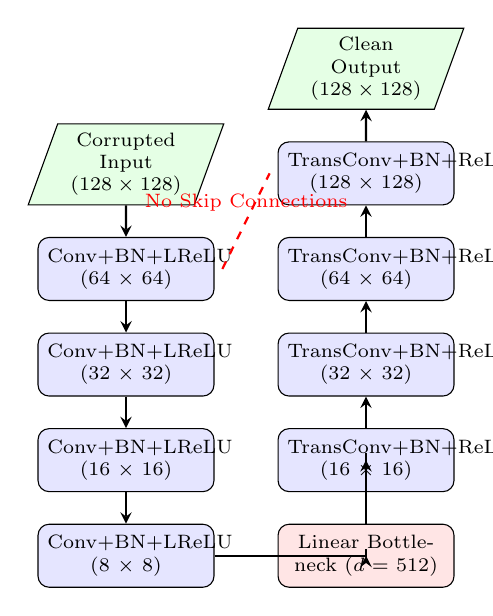
\begin{tikzpicture}[
    node distance=0.4cm and 0.4cm,
    block/.style={rectangle, draw, fill=blue!10, text width=2cm, text centered, rounded corners, minimum height=0.8cm, font=\scriptsize},
    io/.style={trapezium, trapezium left angle=70, trapezium right angle=110, draw, fill=green!10, text width=1.5cm, text centered, minimum height=0.8cm, font=\scriptsize},
    arrow/.style={thick,->,>=stealth}
]
    \node [io] (input) {Corrupted Input ($128\times128$)};
    \node [block, below=of input] (enc1) {Conv+BN+LReLU ($64\times64$)};
    \node [block, below=of enc1] (enc2) {Conv+BN+LReLU ($32\times32$)};
    \node [block, below=of enc2] (enc3) {Conv+BN+LReLU ($16\times16$)};
    \node [block, below=of enc3] (enc4) {Conv+BN+LReLU ($8\times8$)};
    
    \node [block, fill=red!10, right=0.8cm of enc4] (bottleneck) {Linear Bottleneck ($d=512$)};
    
    \node [block, above=of bottleneck] (dec4) {TransConv+BN+ReLU ($16\times16$)};
    \node [block, above=of dec4] (dec3) {TransConv+BN+ReLU ($32\times32$)};
    \node [block, above=of dec3] (dec2) {TransConv+BN+ReLU ($64\times64$)};
    \node [block, above=of dec2] (dec1) {TransConv+BN+ReLU ($128\times128$)};
    \node [io, above=of dec1] (output) {Clean Output ($128\times128$)};

    \draw [arrow] (input) -- (enc1);
    \draw [arrow] (enc1) -- (enc2);
    \draw [arrow] (enc2) -- (enc3);
    \draw [arrow] (enc3) -- (enc4);
    \draw [arrow] (enc4) -| (bottleneck);
    \draw [arrow] (bottleneck) |- (dec4);
    \draw [arrow] (dec4) -- (dec3);
    \draw [arrow] (dec3) -- (dec2);
    \draw [arrow] (dec2) -- (dec1);
    \draw [arrow] (dec1) -- (output);
    
    % Draw boundary for lack of skip connections
    \draw[red, dashed, thick] ($(enc1.east)+(0.1,0)$) -- ($(dec1.west)+(-0.1,0)$) node[midway, above, font=\scriptsize] {No Skip Connections};
\end{tikzpicture}
\caption{Task 1: Universal Autoencoder Architecture.}
\label{fig:arch_task1}
\end{figure}

The universal autoencoder consists of a convolutional encoder, a 1D latent bottleneck, and a convolutional decoder without skip connections.

\textbf{Encoder.} Four convolutional blocks progressively reduce spatial resolution: $128 \rightarrow 64 \rightarrow 32 \rightarrow 16 \rightarrow 8$, using $4 \times 4$ kernels with stride~2 and padding~1. Channel dimensions expand geometrically as $[C, 2C, 4C, 8C]$ where $C$ is the base channel count. Each block applies Batch Normalization~\cite{ioffe2015batch} followed by LeakyReLU($0.2$). The $8 \times 8 \times 8C$ feature map is flattened and projected through a linear layer to a $d$-dimensional bottleneck vector. Dropout is applied before the linear projection.

\textbf{Decoder.} A linear layer maps the bottleneck vector back to the spatial dimensions $8C \times 8 \times 8$. Four transposed convolution blocks symmetrically expand the resolution: $8 \rightarrow 16 \rightarrow 32 \rightarrow 64 \rightarrow 128$, with BatchNorm and ReLU activations. The final layer produces a 3-channel RGB output with a Sigmoid activation to constrain values to $[0, 1]$.

\textbf{Design Justification.} LeakyReLU is used in the encoder to prevent ``dead neuron'' problems during aggressive spatial compression, while standard ReLU suffices in the expanding decoder path. The strict 1D bottleneck---without U-Net-style skip connections---forces the network to discard high-frequency noise and learn a genuinely compressed representation. Transposed convolutions with kernel size~4 and stride~2 avoid checkerboard artifacts through exact divisibility~\cite{odena2016deconvolution}.

\subsection{Loss Function}

The combined reconstruction loss is:
\begin{equation}
\mathcal{L}_{\text{task1}} = \alpha \cdot \mathcal{L}_{\text{L1}}(x, \hat{x}) + (1 - \alpha) \cdot (1 - \text{SSIM}(x, \hat{x}))
\label{eq:task1_loss}
\end{equation}
where $\alpha$ is a learnable trade-off parameter optimized by Optuna. L1 encourages pixel-accurate reconstruction, while the SSIM component preserves structural patterns, edges, and local contrast. The SSIM implementation uses \texttt{torchmetrics} with a data range of~1.0.

\subsection{Hyperparameter Optimization}

An Optuna study with 20 trials, using the Tree-structured Parzen Estimator (TPE) sampler and MedianPruner (5 startup trials, 5 warmup steps), searched the following space:

\begin{table}[H]
\centering
\caption{Task 1 Optuna Search Space and Best Configuration}
\label{tab:task1_hpo}
\begin{tabular}{lcc}
\toprule
\textbf{Parameter} & \textbf{Search Range} & \textbf{Best Value} \\
\midrule
Learning rate & $[10^{-5}, 10^{-2}]$ (log) & $1.13 \times 10^{-4}$ \\
Batch size & $\{16, 32, 64\}$ & 32 \\
Bottleneck dim & $[64, 512]$ step 64 & 512 \\
Base channels & $\{32, 48, 64\}$ & 48 \\
Dropout & $[0.0, 0.5]$ & 0.026 \\
Alpha ($\alpha$) & $[0.5, 1.0]$ & 0.958 \\
\bottomrule
\end{tabular}
\end{table}

The best trial (\#14) achieved a validation loss of 0.0900. The high $\alpha = 0.958$ indicates that the network heavily favored L1 reconstruction over SSIM, which is consistent with the observation that over-weighting SSIM can cause structural hallucinations in bottleneck autoencoders. Training used Adam optimization with early stopping (patience~5, $\delta = 0.001$) over a maximum of 30 epochs.

\subsection{Experimental Results}

The final model was evaluated on 36,690 deterministic test samples.

\begin{table}[H]
\centering
\caption{Task 1: Per-Corruption Results (Test Set)}
\label{tab:task1_corruption}
\begin{tabular}{lcc}
\toprule
\textbf{Corruption Type} & \textbf{L1 $\downarrow$} & \textbf{SSIM $\uparrow$} \\
\midrule
Clean (baseline) & 0.0701 & 0.5137 \\
Gaussian Blur & \textbf{0.0699} & \textbf{0.5126} \\
Salt \& Pepper & 0.0712 & 0.5077 \\
Rectangular Occlusion & 0.0836 & 0.4715 \\
\bottomrule
\end{tabular}
\end{table}

\begin{table}[H]
\centering
\caption{Task 1: Per-Severity Results (Test Set)}
\label{tab:task1_severity}
\begin{tabular}{lcc}
\toprule
\textbf{Severity} & \textbf{L1 $\downarrow$} & \textbf{SSIM $\uparrow$} \\
\midrule
Low & 0.0721 & 0.5061 \\
Medium & 0.0744 & 0.4984 \\
High & 0.0781 & 0.4872 \\
\bottomrule
\end{tabular}
\end{table}

\textbf{Analysis.} The model performs comparably on clean, blurred, and noisy inputs, demonstrating that the bottleneck architecture can effectively resolve local, high-frequency spatial degradations. Performance degrades most significantly for rectangular occlusion, which requires the model to semantically hallucinate entirely missing structural information---a task beyond the capacity of a strict bottleneck autoencoder. As expected, L1 increases and SSIM decreases monotonically with corruption severity.

\textbf{Failure Cases.} The four worst-performing test instances (selected by the exact combined loss function) involve large rectangular occlusions covering critical facial features (e.g., eyes, snout), where the network produces visible blurring artifacts in the reconstructed region. Visual grids of 12 representative examples and 4 failure cases are included in the supplementary materials.

% Fig placeholder — replace path as needed
\begin{figure}[H]
\centering
\begin{subfigure}{0.48\columnwidth}
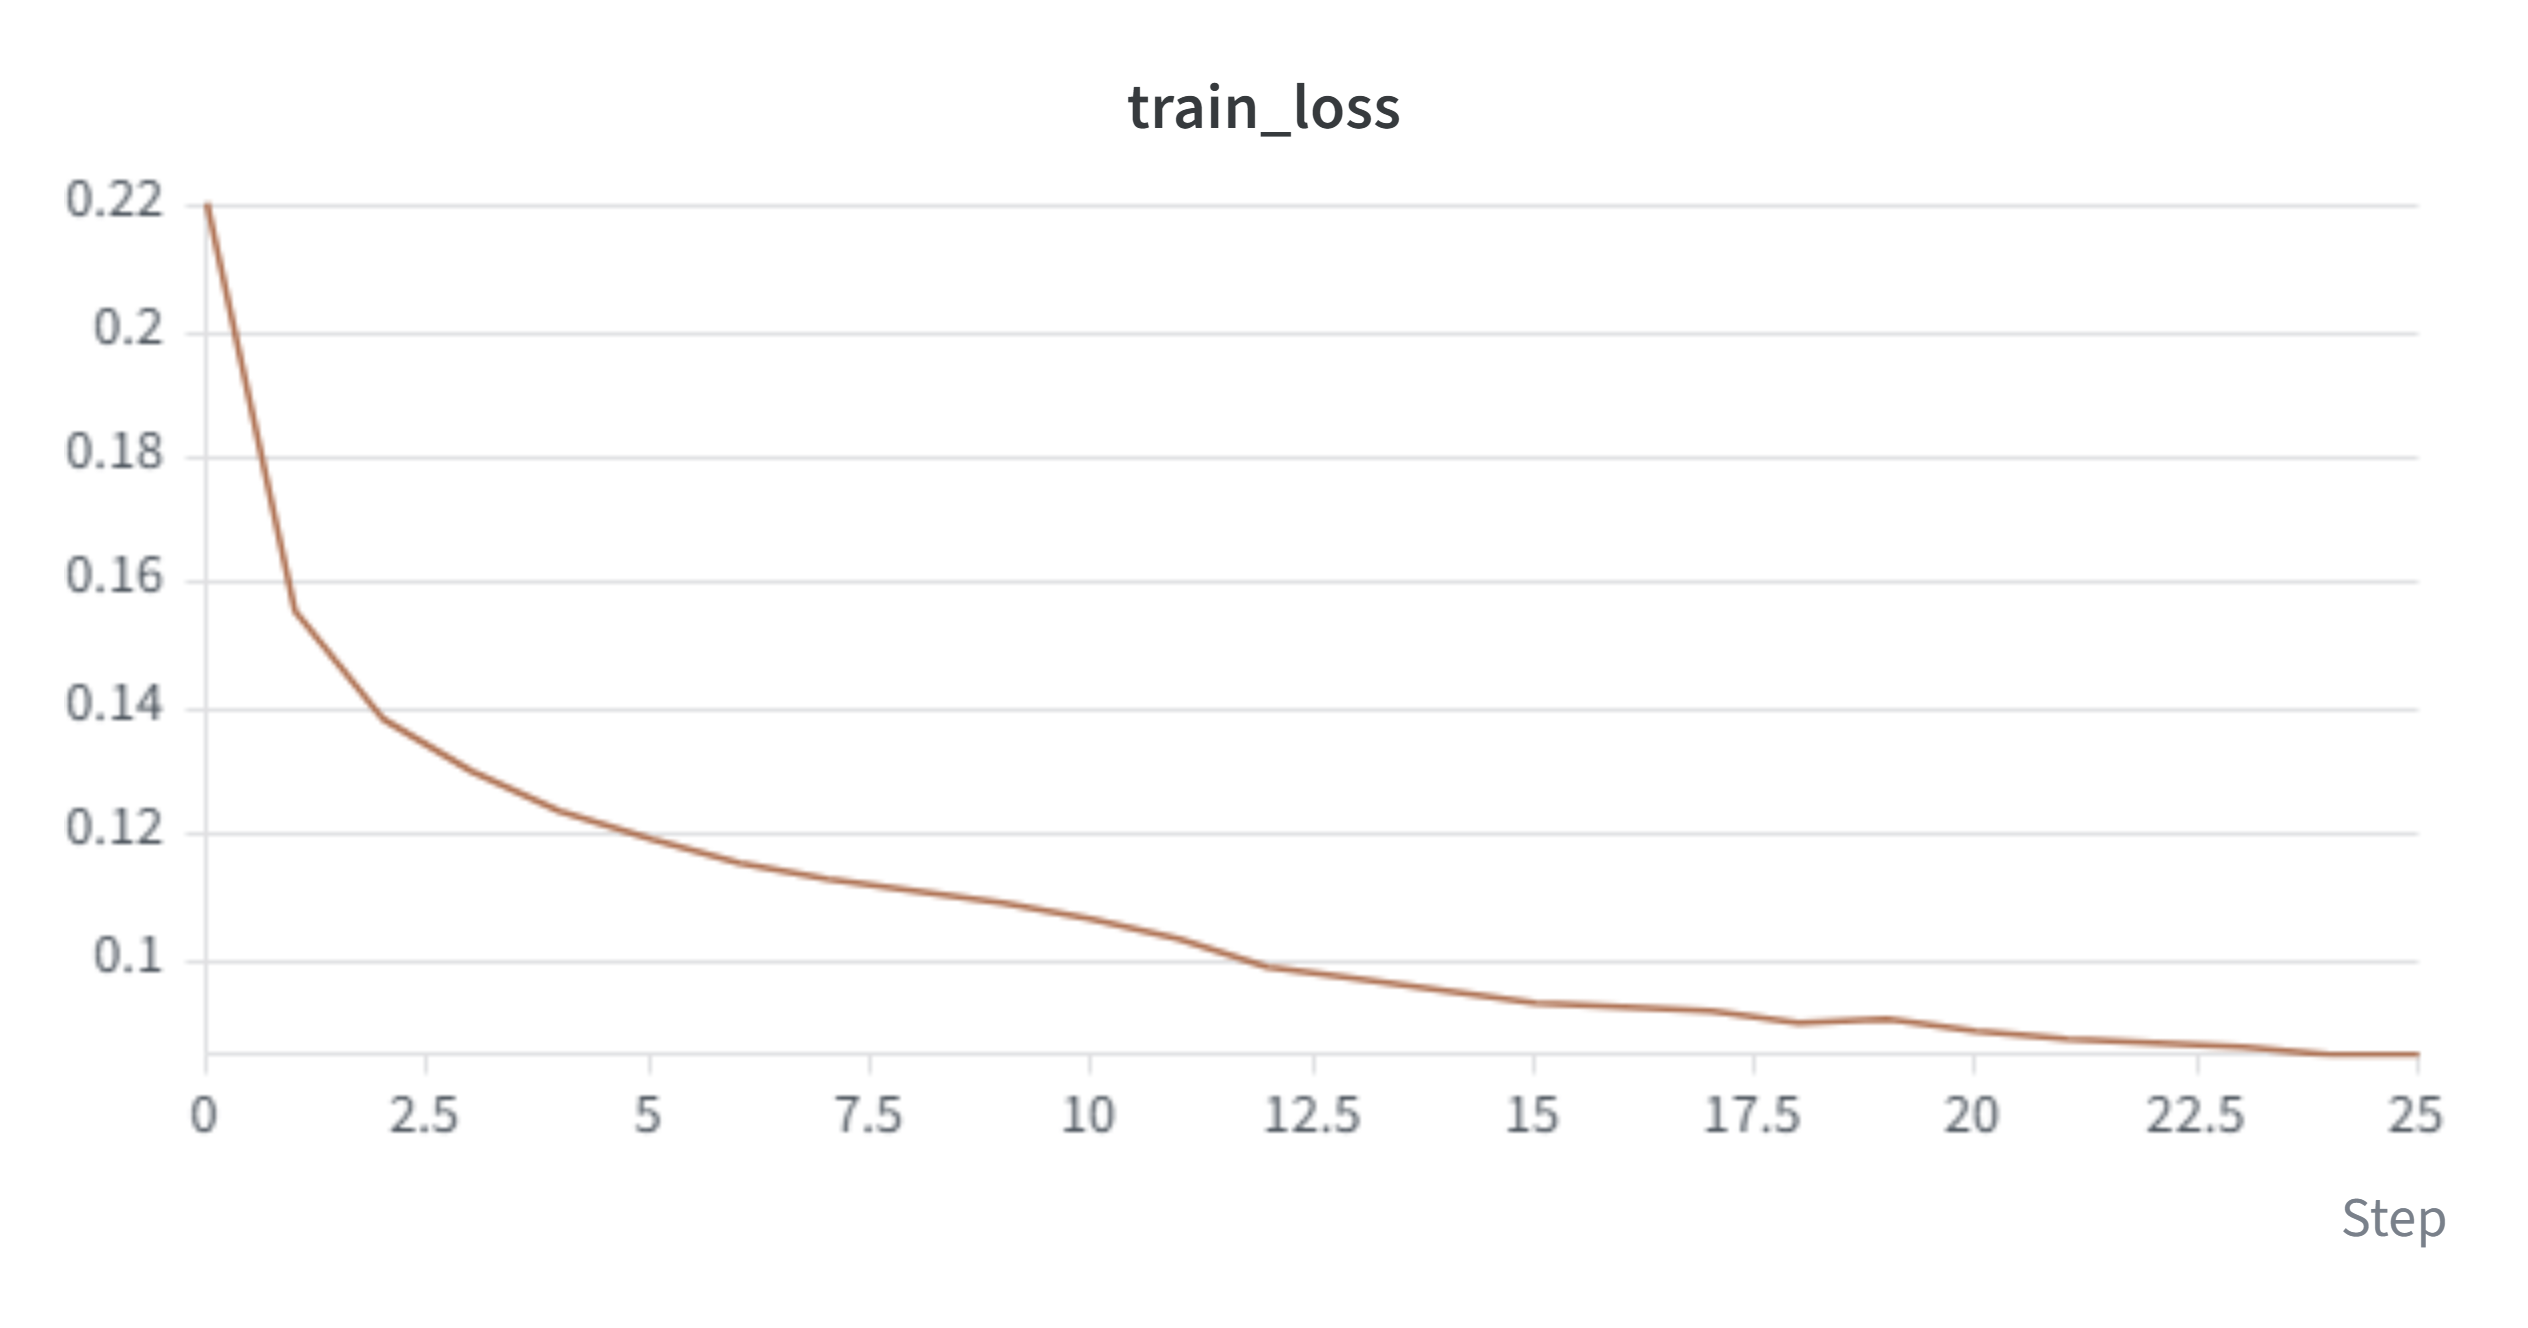
\includegraphics[width=\linewidth]{task1_train_loss.png}
\caption{Training Loss}
\end{subfigure}\hfill
\begin{subfigure}{0.48\columnwidth}
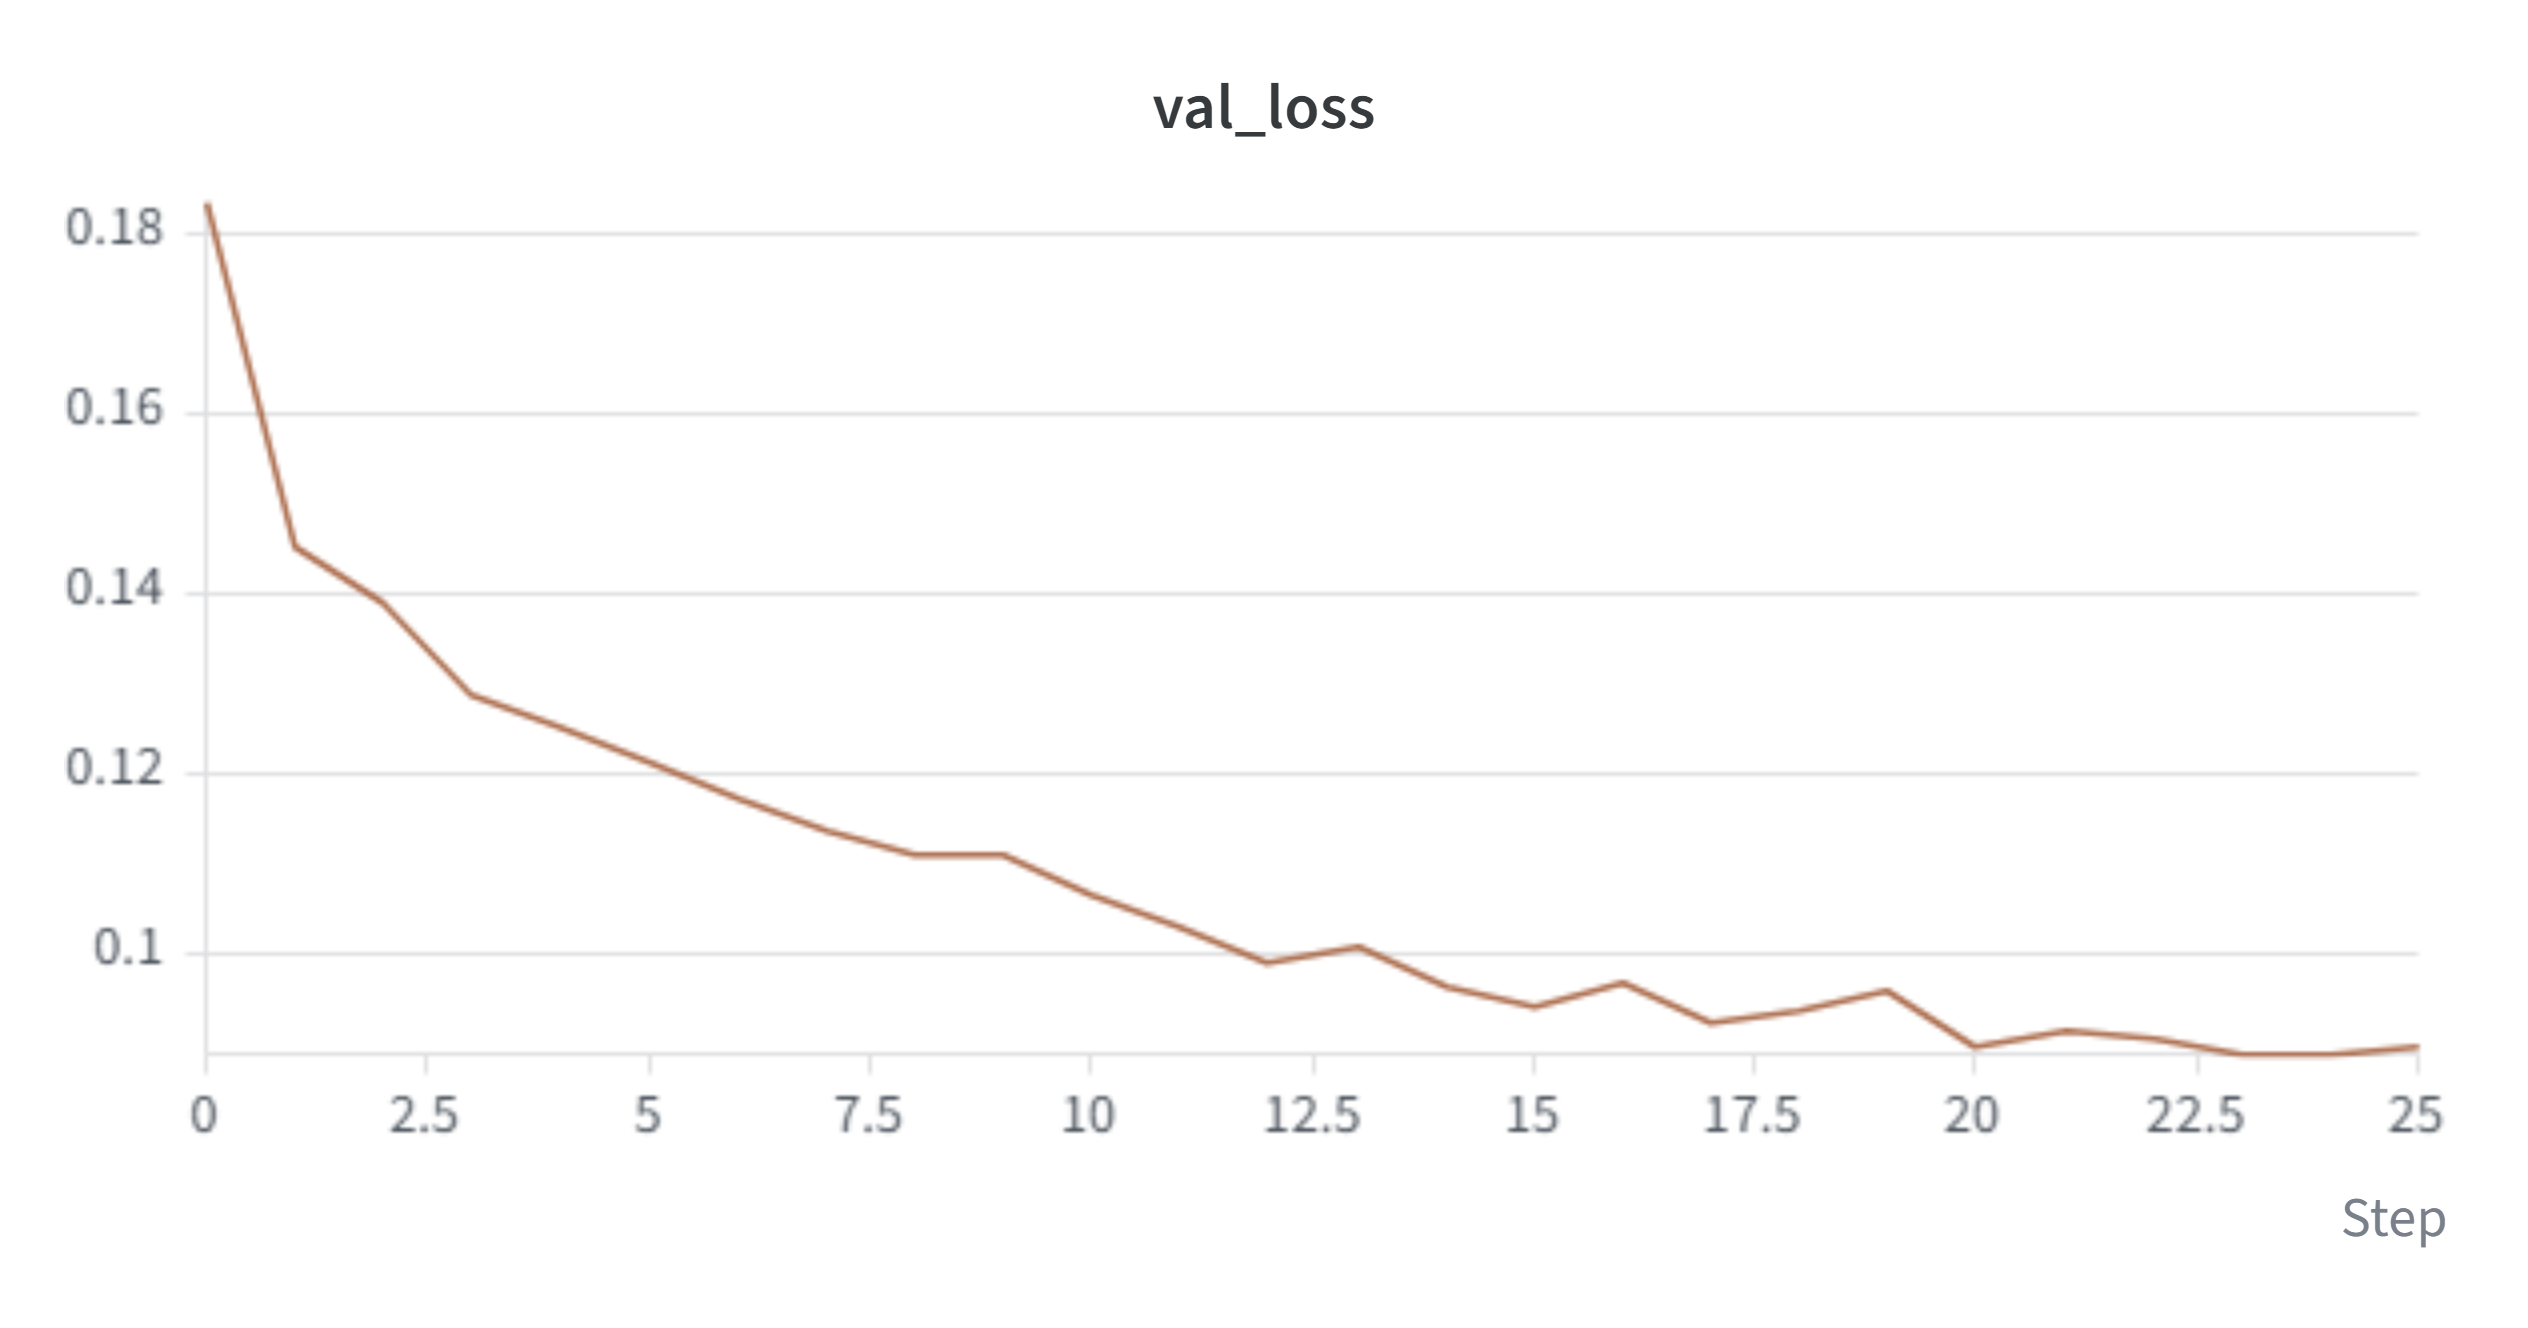
\includegraphics[width=\linewidth]{task1_val_loss.png}
\caption{Validation Loss}
\end{subfigure}
\caption{Task 1: Combined (L1 + SSIM) Loss vs Epoch for the best Optuna trial (\#14). Both curves demonstrate stable convergence without overfitting.}
\label{fig:task1_curves}
\end{figure}
\begin{figure}[H]
\centering
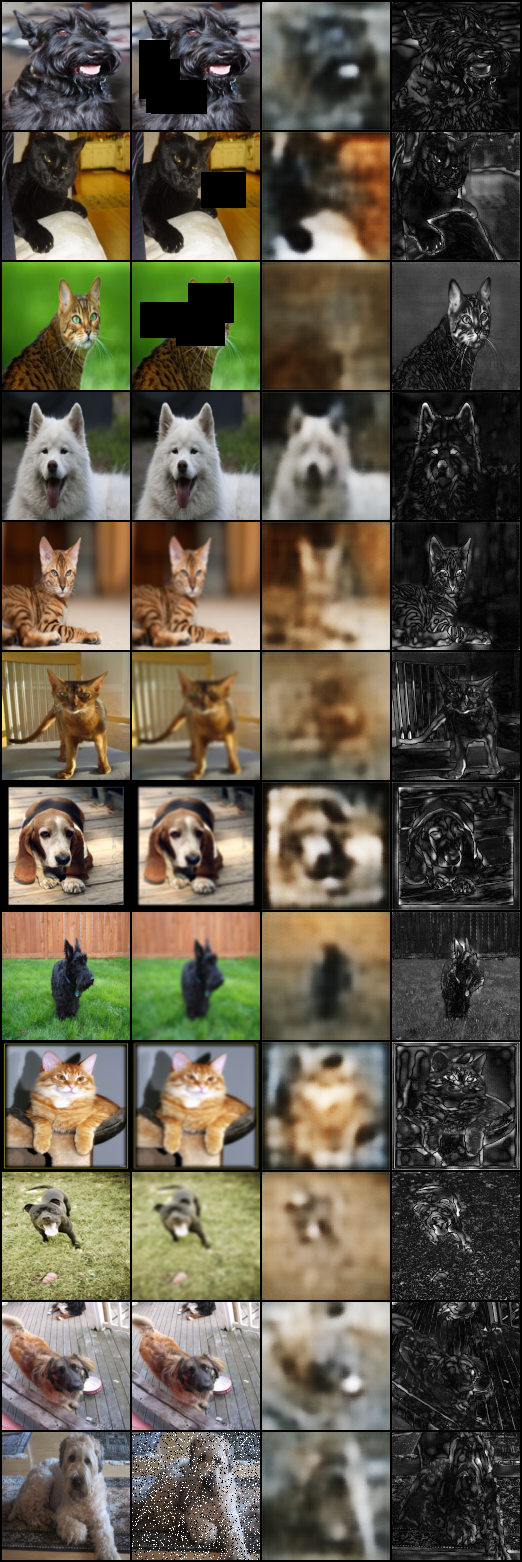
\includegraphics[width=\columnwidth]{task1/representative_examples.png}
\caption{Task 1: Representative reconstruction results. Each row: clean target, corrupted input, reconstruction, absolute error map.}
\label{fig:task1_examples}
\end{figure}

\begin{figure}[H]
\centering
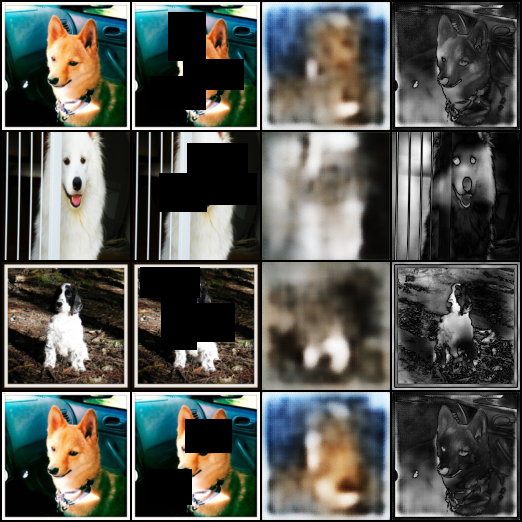
\includegraphics[width=\columnwidth]{task1/failure_cases.png}
\caption{Task 1: Failure cases with highest combined loss, predominantly involving large rectangular occlusions.}
\label{fig:task1_failures}
\end{figure}

% ============================================================
\section{Task 2: Corruption Classification and Hard-Routed Specialist Autoencoders}
\label{sec:task2}

\subsection{Corruption Classifier}

\subsubsection{Architecture}

\begin{figure}[H]
\centering
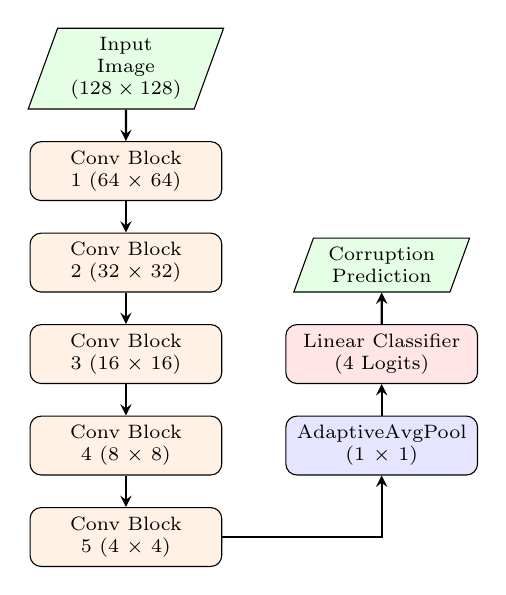
\begin{tikzpicture}[
    node distance=0.4cm and 0.5cm,
    block/.style={rectangle, draw, fill=orange!10, text width=2.2cm, text centered, rounded corners, minimum height=0.6cm, font=\scriptsize},
    io/.style={trapezium, trapezium left angle=70, trapezium right angle=110, draw, fill=green!10, text width=1.5cm, text centered, minimum height=0.6cm, font=\scriptsize},
    arrow/.style={thick,->,>=stealth}
]
    \node [io] (input) {Input Image ($128\times128$)};
    \node [block, below=of input] (conv1) {Conv Block 1 ($64\times64$)};
    \node [block, below=of conv1] (conv2) {Conv Block 2 ($32\times32$)};
    \node [block, below=of conv2] (conv3) {Conv Block 3 ($16\times16$)};
    \node [block, below=of conv3] (conv4) {Conv Block 4 ($8\times8$)};
    \node [block, below=of conv4] (conv5) {Conv Block 5 ($4\times4$)};
    
    \node [block, fill=blue!10, right=0.8cm of conv4] (pool) {AdaptiveAvgPool ($1\times1$)};
    \node [block, fill=red!10, above=of pool] (fc) {Linear Classifier (4 Logits)};
    \node [io, above=of fc] (output) {Corruption Prediction};

    \draw [arrow] (input) -- (conv1);
    \draw [arrow] (conv1) -- (conv2);
    \draw [arrow] (conv2) -- (conv3);
    \draw [arrow] (conv3) -- (conv4);
    \draw [arrow] (conv4) -- (conv5);
    \draw [arrow] (conv5) -| (pool);
    \draw [arrow] (pool) -- (fc);
    \draw [arrow] (fc) -- (output);
\end{tikzpicture}
\caption{Task 2: Corruption Classifier Architecture with Adaptive Pooling.}
\label{fig:arch_task2}
\end{figure}

The classifier uses 5 convolutional blocks that progressively halve spatial resolution ($128 \rightarrow 64 \rightarrow 32 \rightarrow 16 \rightarrow 8 \rightarrow 4$) using $3 \times 3$ kernels with stride~2 and padding~1, with channel expansion $[C, 2C, 4C, 8C, 8C]$. Each block applies BatchNorm and LeakyReLU($0.2$). An Adaptive Average Pooling layer reduces the final feature map to $1 \times 1$, making the classifier spatially invariant---critical for detecting rectangular occlusions regardless of mask position. The classification head applies dropout followed by a linear projection to 4 logits (clean, salt-and-pepper, Gaussian blur, rectangular occlusion).

\subsubsection{Loss and Training}
The classifier is trained with cross-entropy loss using Adam with weight decay. The custom balanced collate function guarantees uniform class distribution in every batch.

\subsubsection{Hyperparameter Optimization}

\begin{table}[H]
\centering
\caption{Task 2 Classifier: Optuna Search Space}
\label{tab:task2_cls_hpo}
\begin{tabular}{lc}
\toprule
\textbf{Parameter} & \textbf{Search Range} \\
\midrule
Learning rate & $[10^{-5}, 10^{-2}]$ (log) \\
Batch size & $\{16, 32, 64\}$ \\
Base channels & $\{16, 32, 64\}$ \\
Dropout & $[0.0, 0.5]$ \\
Weight decay & $[10^{-6}, 10^{-2}]$ (log) \\
\bottomrule
\end{tabular}
\end{table}

Optuna was configured to minimize the validation cross-entropy loss, which provides a smoother optimization landscape than accuracy. 20 trials were executed with the best trial (\#20) identified via early stopping with patience~5.

\subsubsection{Classification Results}

\begin{table}[H]
\centering
\caption{Task 2 Classifier: Test Set Metrics (N=36,690)}
\label{tab:task2_cls_results}
\begin{tabular}{lc}
\toprule
\textbf{Metric} & \textbf{Value} \\
\midrule
Overall Accuracy & 98.26\% \\
Macro Precision & 96.65\% \\
Macro Recall & 97.88\% \\
Macro F1-Score & 97.21\% \\
\bottomrule
\end{tabular}
\end{table}

\begin{table}[H]
\centering
\caption{Task 2 Classifier: Per-Class F1-Scores}
\label{tab:task2_cls_perclass}
\begin{tabular}{lc}
\toprule
\textbf{Corruption Class} & \textbf{F1-Score} \\
\midrule
Clean & 91.89\% \\
Salt \& Pepper & 99.98\% \\
Gaussian Blur & 99.41\% \\
Rectangular Occlusion & 97.57\% \\
\bottomrule
\end{tabular}
\end{table}

The classifier achieves near-perfect detection of artificial corruptions ($>$99\% F1 for salt-and-pepper and blur). The slightly lower F1 for the ``clean'' class (91.89\%) occurs because extremely subtle corruptions (e.g., blur with $\sigma = 0.5$) are occasionally misclassified as clean, which is an acceptable trade-off since it triggers the identity bypass rather than unnecessary restoration processing.

\begin{figure}[H]
\centering
\begin{subfigure}{0.48\columnwidth}
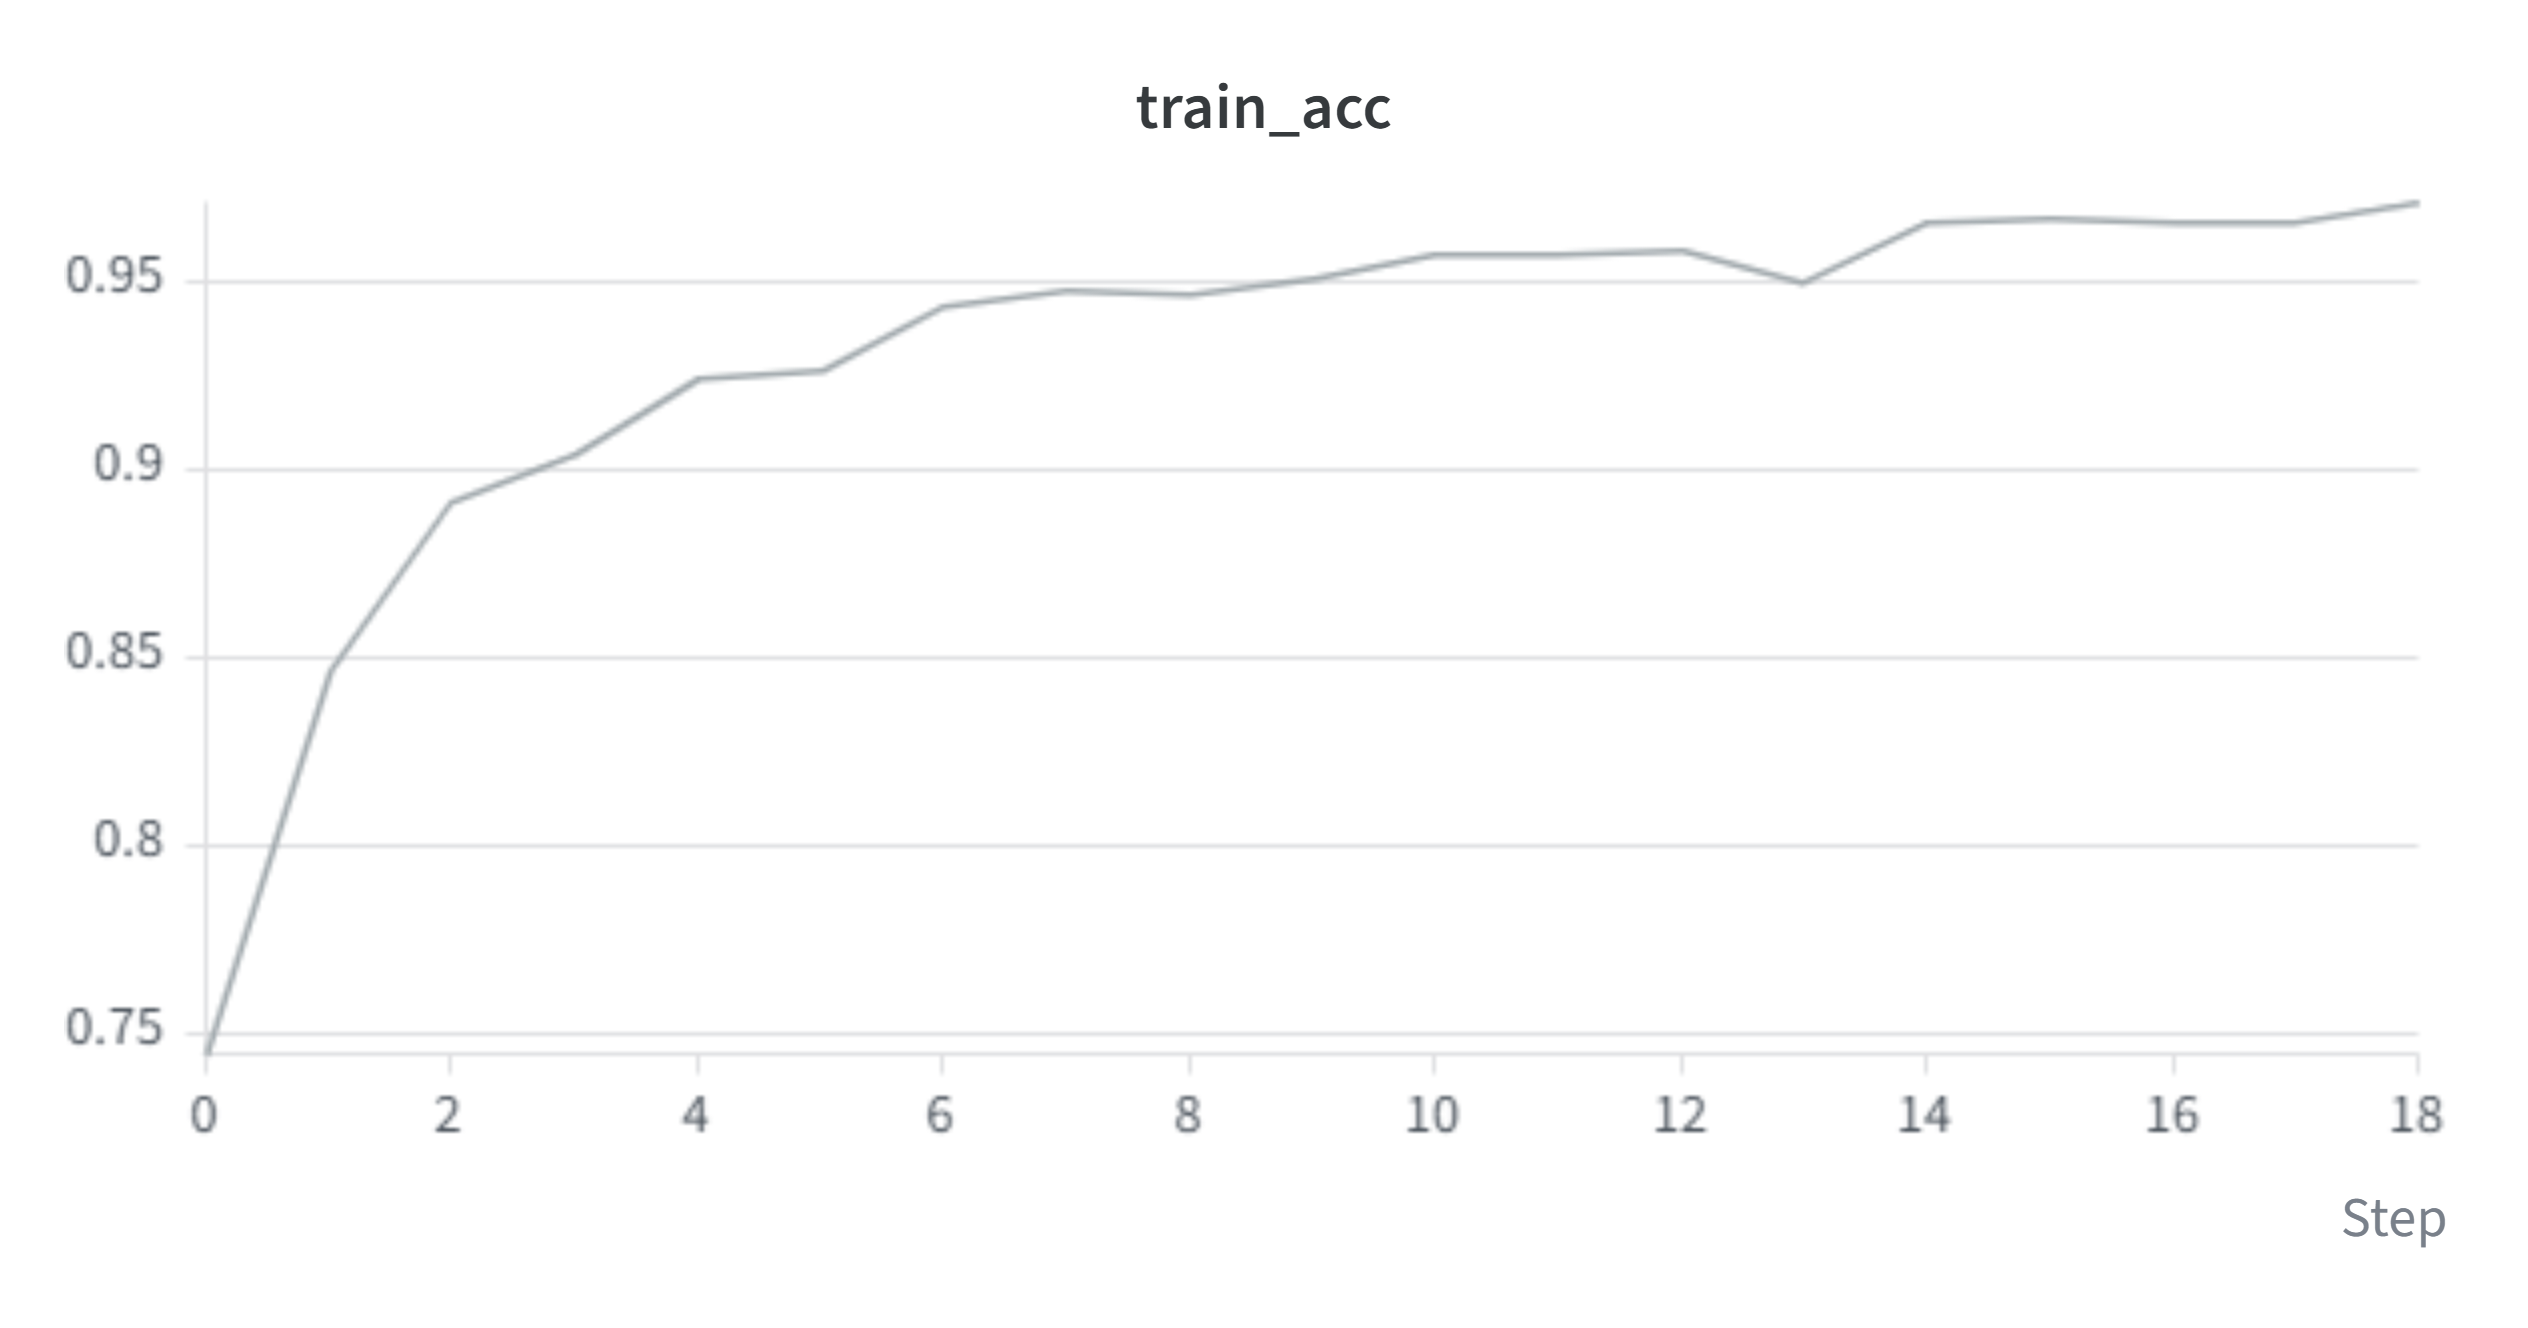
\includegraphics[width=\linewidth]{task2_cls_train_accuracy.png}
\caption{Training Accuracy}
\end{subfigure}\hfill
\begin{subfigure}{0.48\columnwidth}
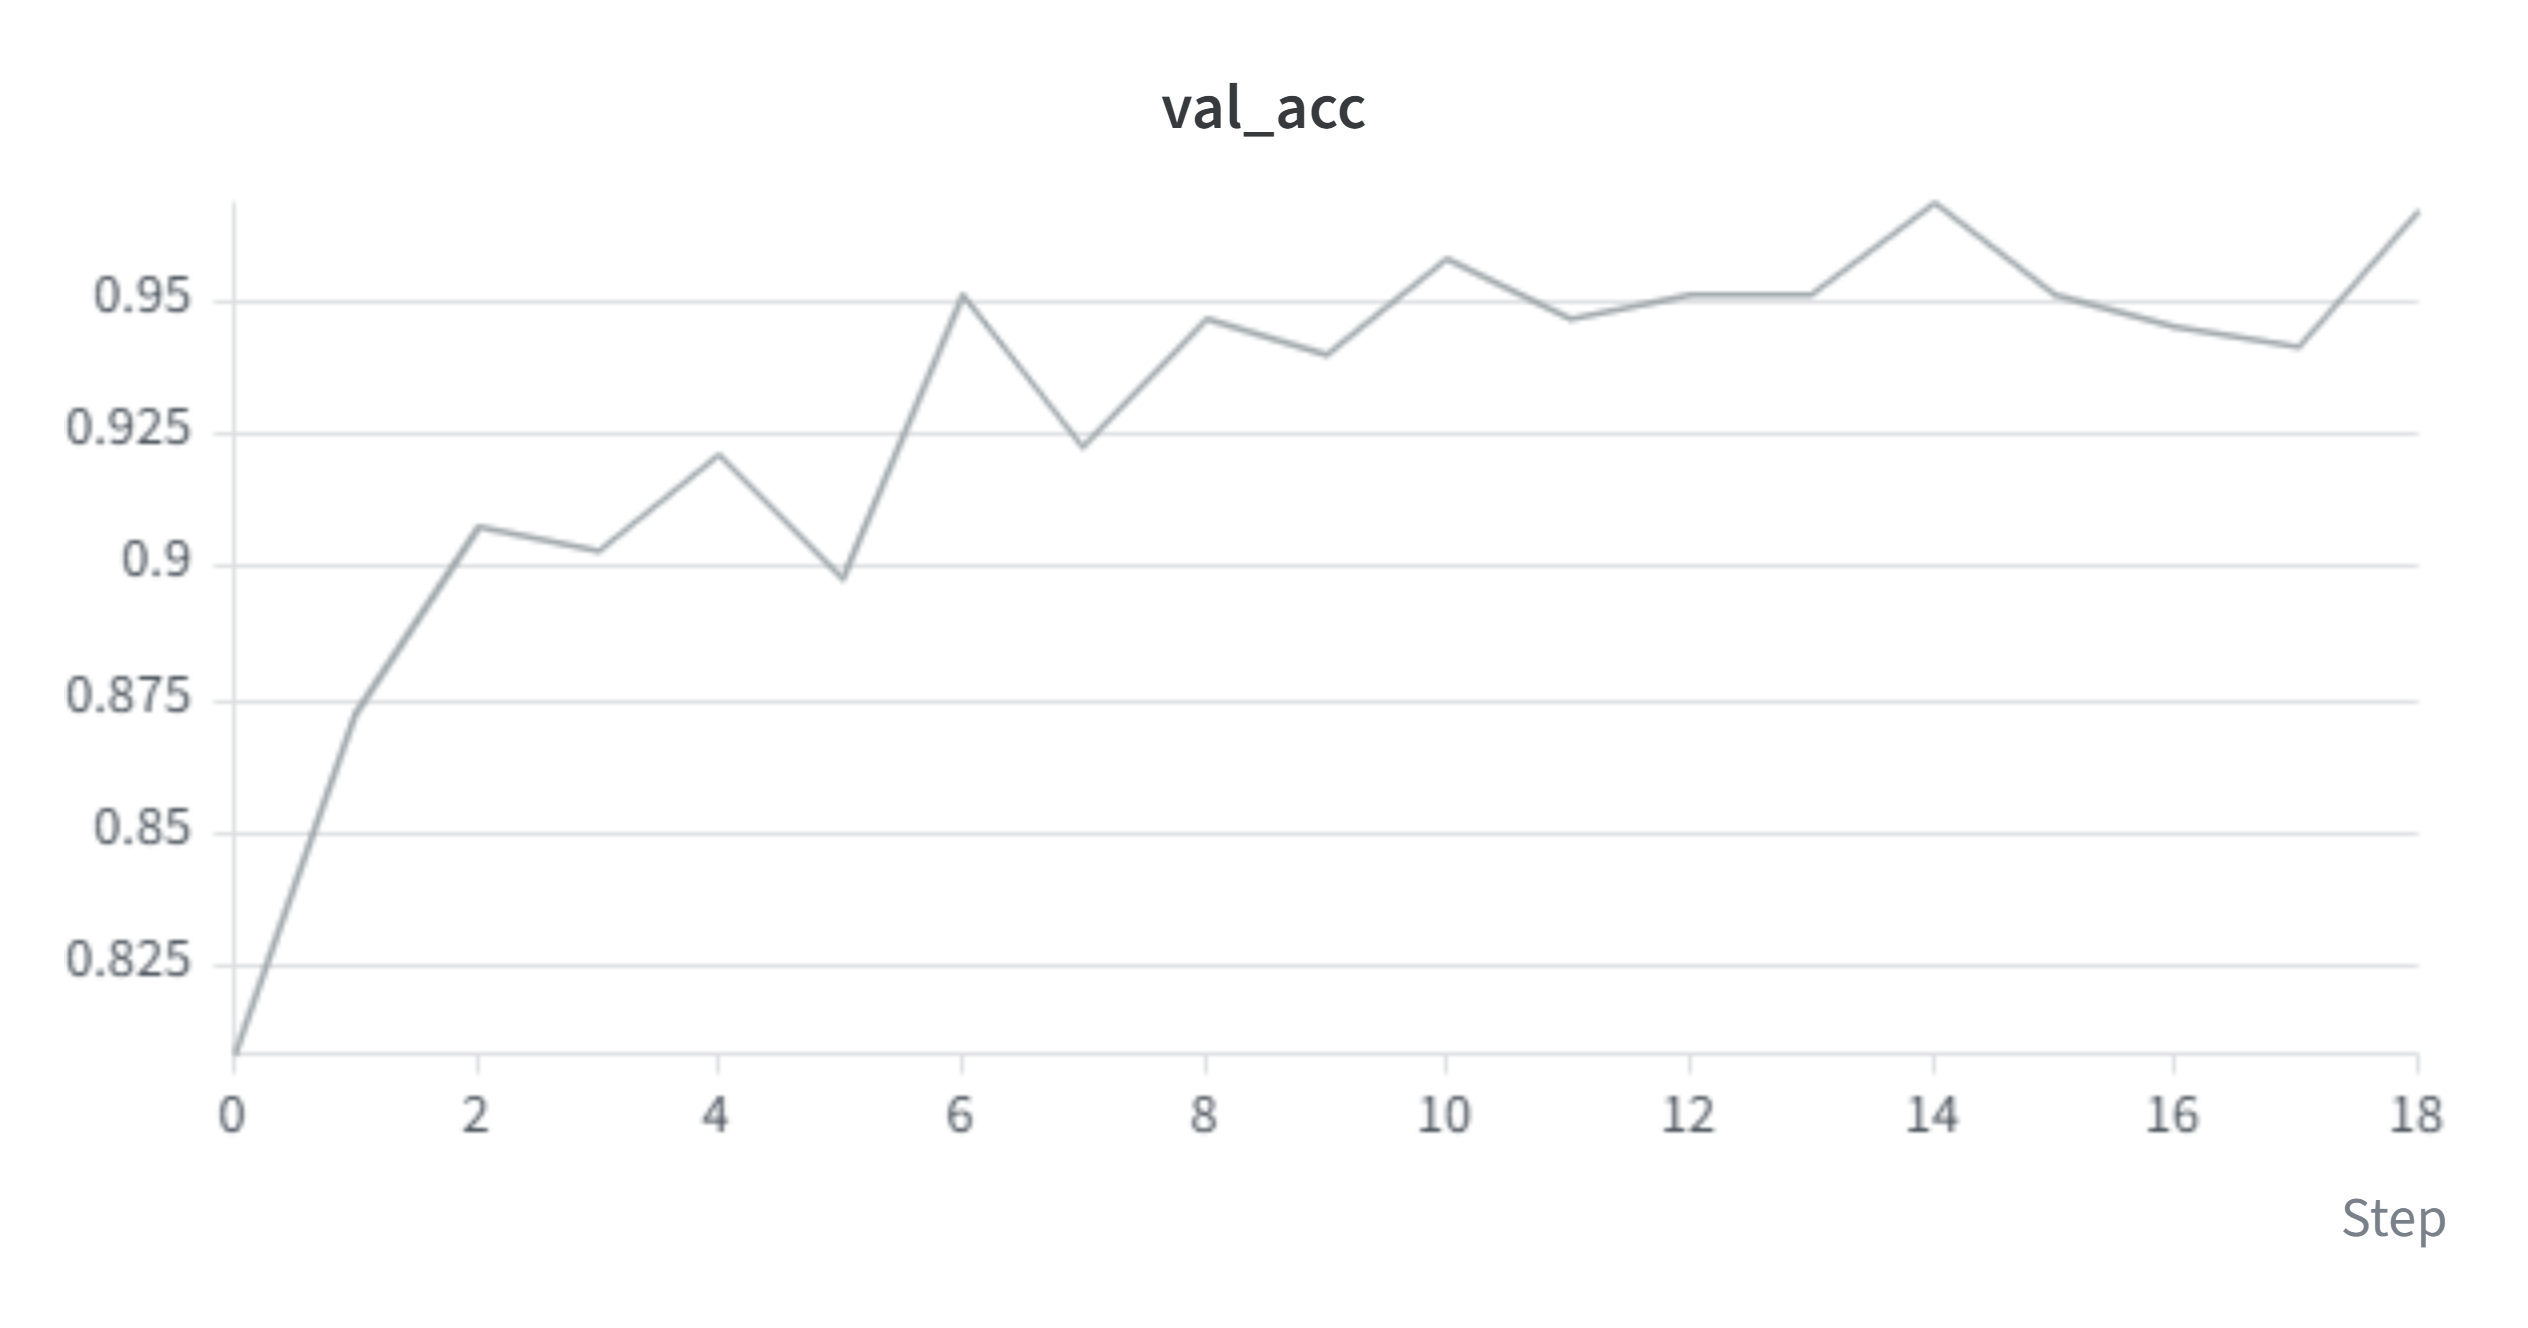
\includegraphics[width=\linewidth]{task2_cls_val_accuracy.png}
\caption{Validation Accuracy}
\end{subfigure}
\caption{Task 2: Classifier Accuracy vs Epoch. The model rapidly approaches near-perfect accuracy on both sets, indicating the spatial invariance (Adaptive Pooling) effectively captures corruption signatures.}
\label{fig:task2_curves}
\end{figure}

\begin{figure}[H]
\centering
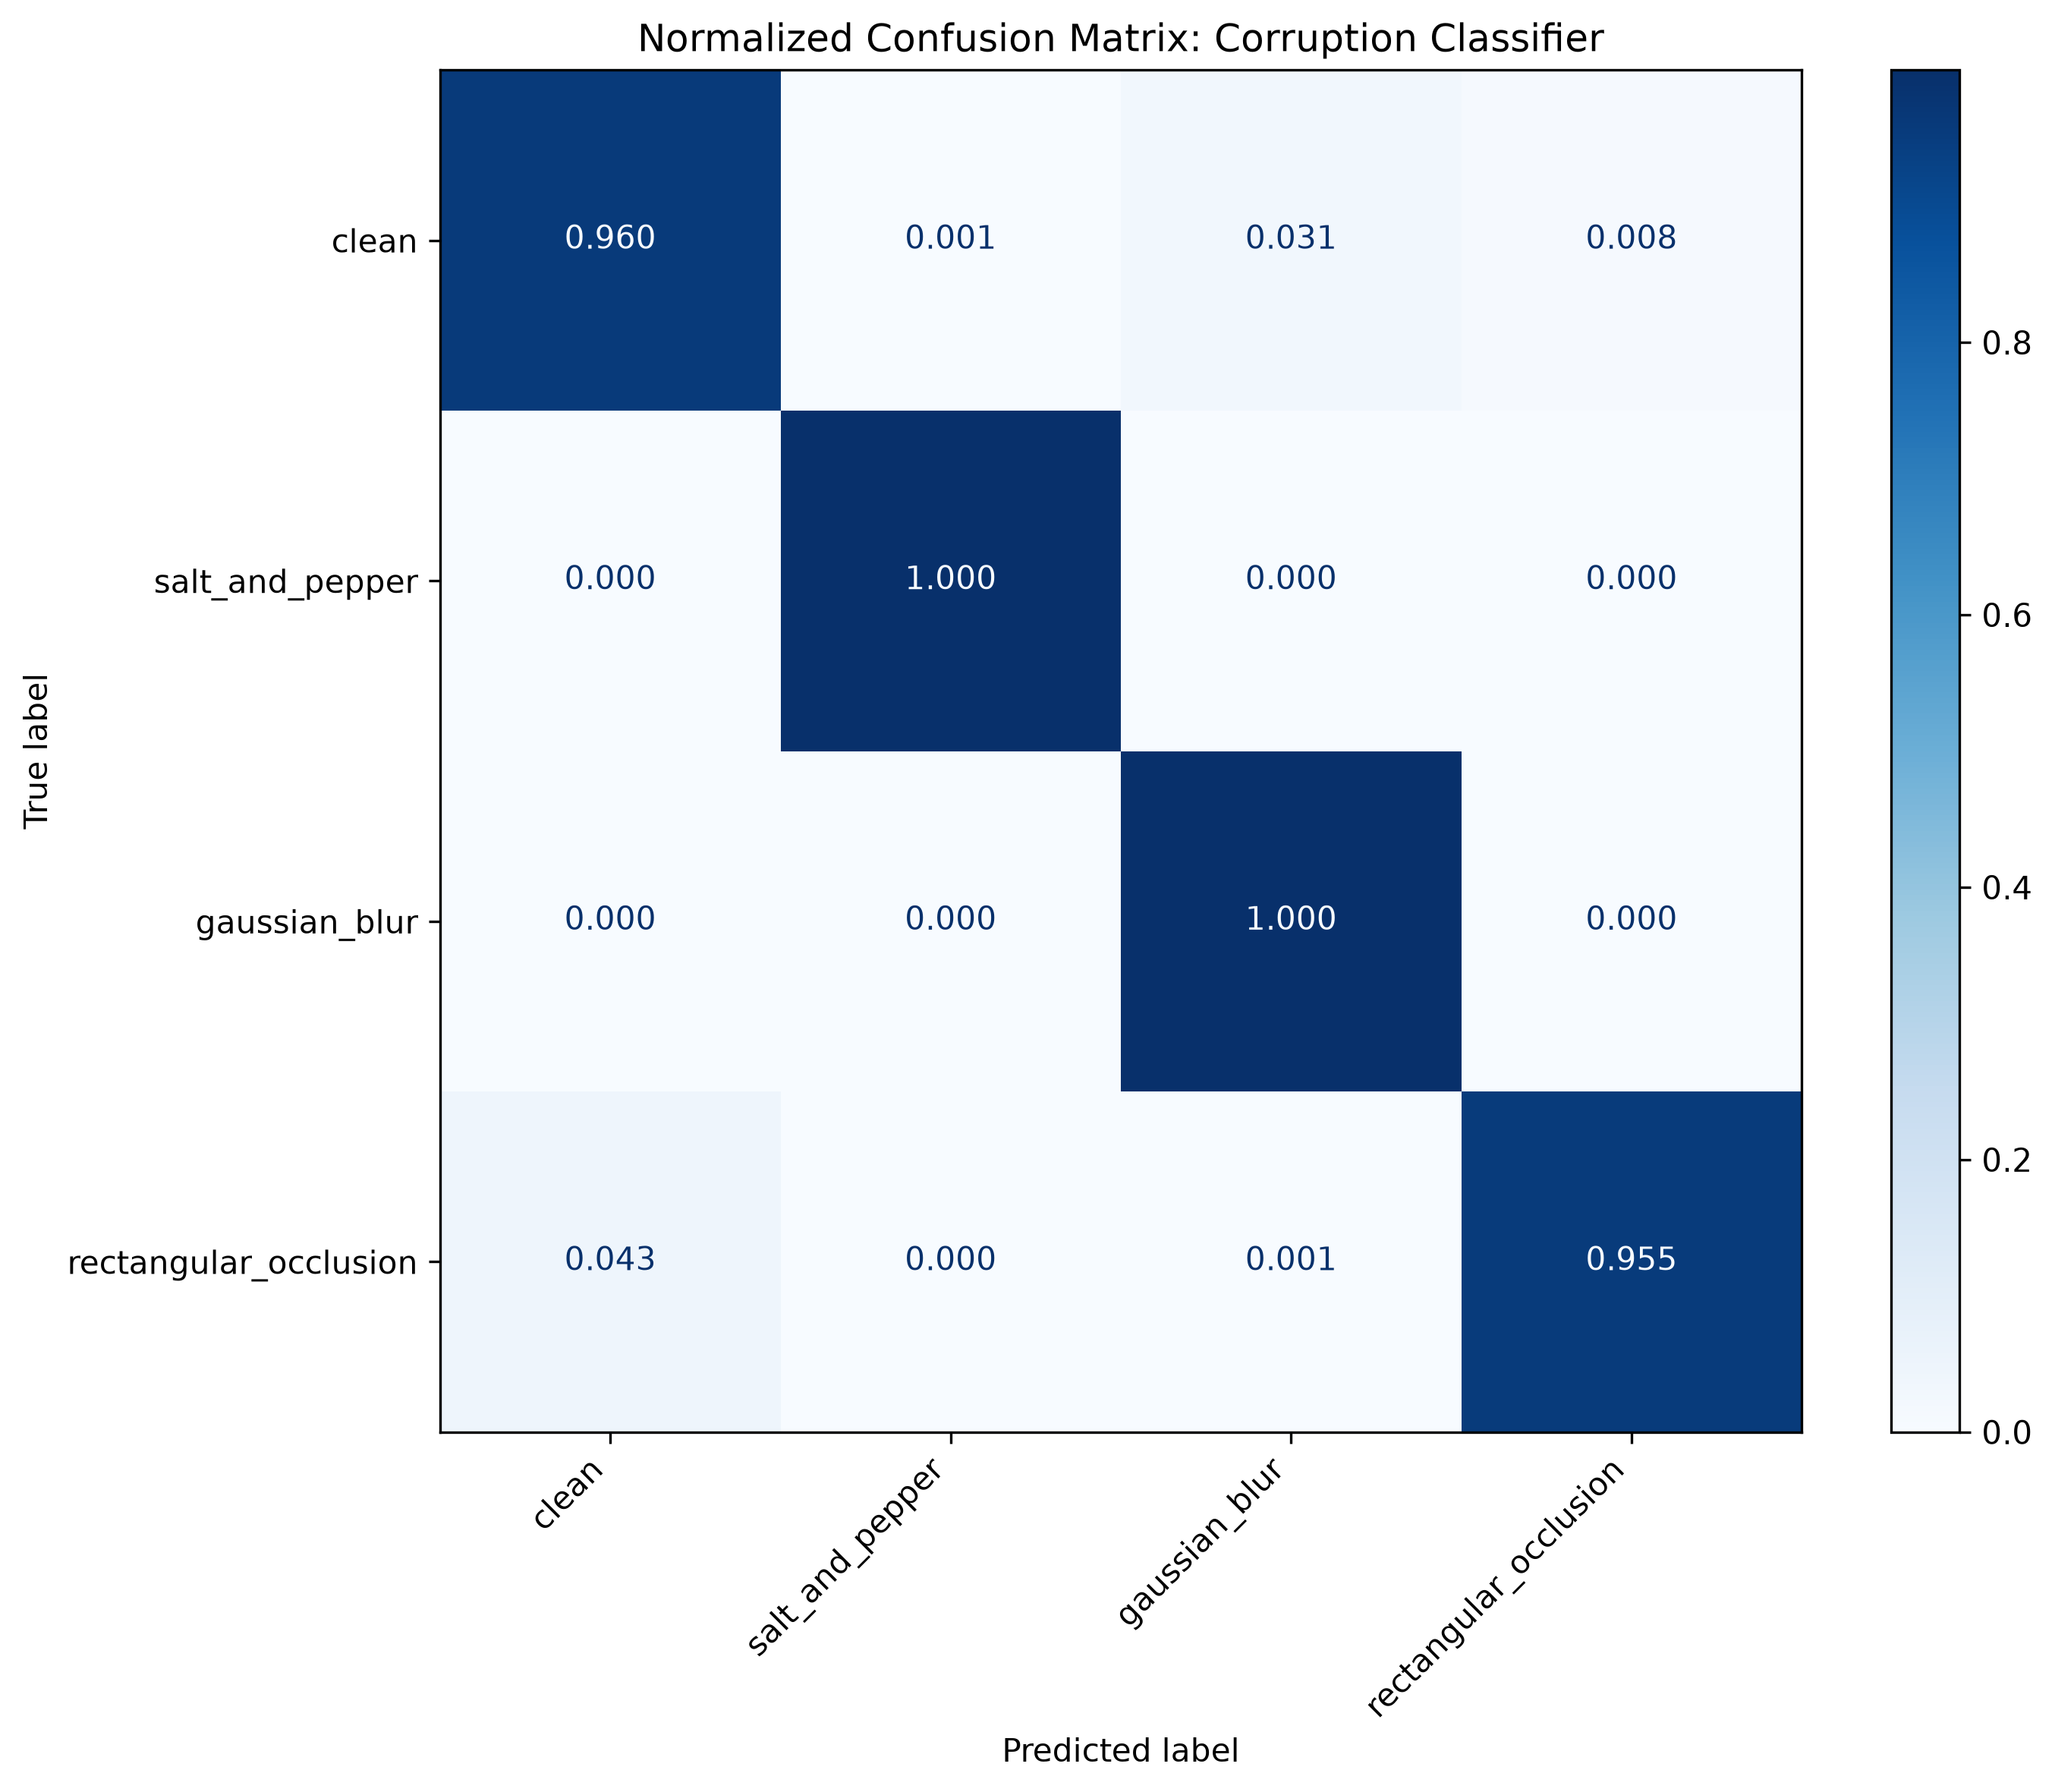
\includegraphics[width=0.7\columnwidth]{task2/classifier_confusion_matrix.png}
\caption{Task 2: Normalized 4-class confusion matrix showing high diagonal accuracy and slight overlap between clean and low-severity corruptions.}
\label{fig:task2_confusion}
\end{figure}

\subsection{Specialist Autoencoders}

Three specialist autoencoders---one each for salt-and-pepper, Gaussian blur, and rectangular occlusion---reuse the \texttt{UniversalAutoencoder} architecture from Task~1 with independently trained parameters. A shared Optuna search (20 trials, 15 epochs each, 3 simultaneous micro-models per trial) identified the common architecture, after which each specialist was trained independently for up to 100 epochs to prevent VRAM exhaustion.

\begin{table}[H]
\centering
\caption{Task 2 Specialists: Shared Optuna Search Space}
\label{tab:task2_spec_hpo}
\begin{tabular}{lc}
\toprule
\textbf{Parameter} & \textbf{Search Range} \\
\midrule
Learning rate & $[10^{-5}, 10^{-2}]$ (log) \\
Bottleneck dim & $[64, 512]$ step 64 \\
Base channels & $\{32, 48, 64\}$ \\
Batch size & $\{16, 32, 64\}$ \\
Alpha ($\alpha$) & $[0.5, 1.0]$ \\
\bottomrule
\end{tabular}
\end{table}

\subsection{Hard-Routed Inference}

During inference, the classifier first predicts the corruption type. If ``clean'' is predicted, the identity bypass returns the input unchanged. Otherwise, the corresponding specialist processes the image:
\begin{equation}
\hat{x} = \begin{cases}
x_c, & r = \text{clean} \\
A_{\text{sp}}(x_c), & r = \text{salt} \\
A_{\text{blur}}(x_c), & r = \text{blur} \\
A_{\text{occ}}(x_c), & r = \text{occlusion}
\end{cases}
\end{equation}

\begin{table}[H]
\centering
\caption{Task 2: Hard-Routed Inference Results (N=36,690)}
\label{tab:task2_routing}
\begin{tabular}{lcc}
\toprule
\textbf{Routing Mode} & \textbf{L1 $\downarrow$} & \textbf{SSIM $\uparrow$} \\
\midrule
Oracle (ground truth) & 0.06814 & 0.53327 \\
Predicted (classifier) & \textbf{0.06774} & \textbf{0.53699} \\
\bottomrule
\end{tabular}
\end{table}

\textbf{Anomaly Analysis.} Interestingly, predicted routing marginally outperforms oracle routing. This counterintuitive result occurs because the classifier occasionally misroutes subtle corruptions (e.g., blur with $\sigma = 0.5$) to the identity bypass, which preserves the original sharp pixels better than forcing the image through a specialist that may over-smooth an already near-clean image.

\begin{figure}[H]
\centering
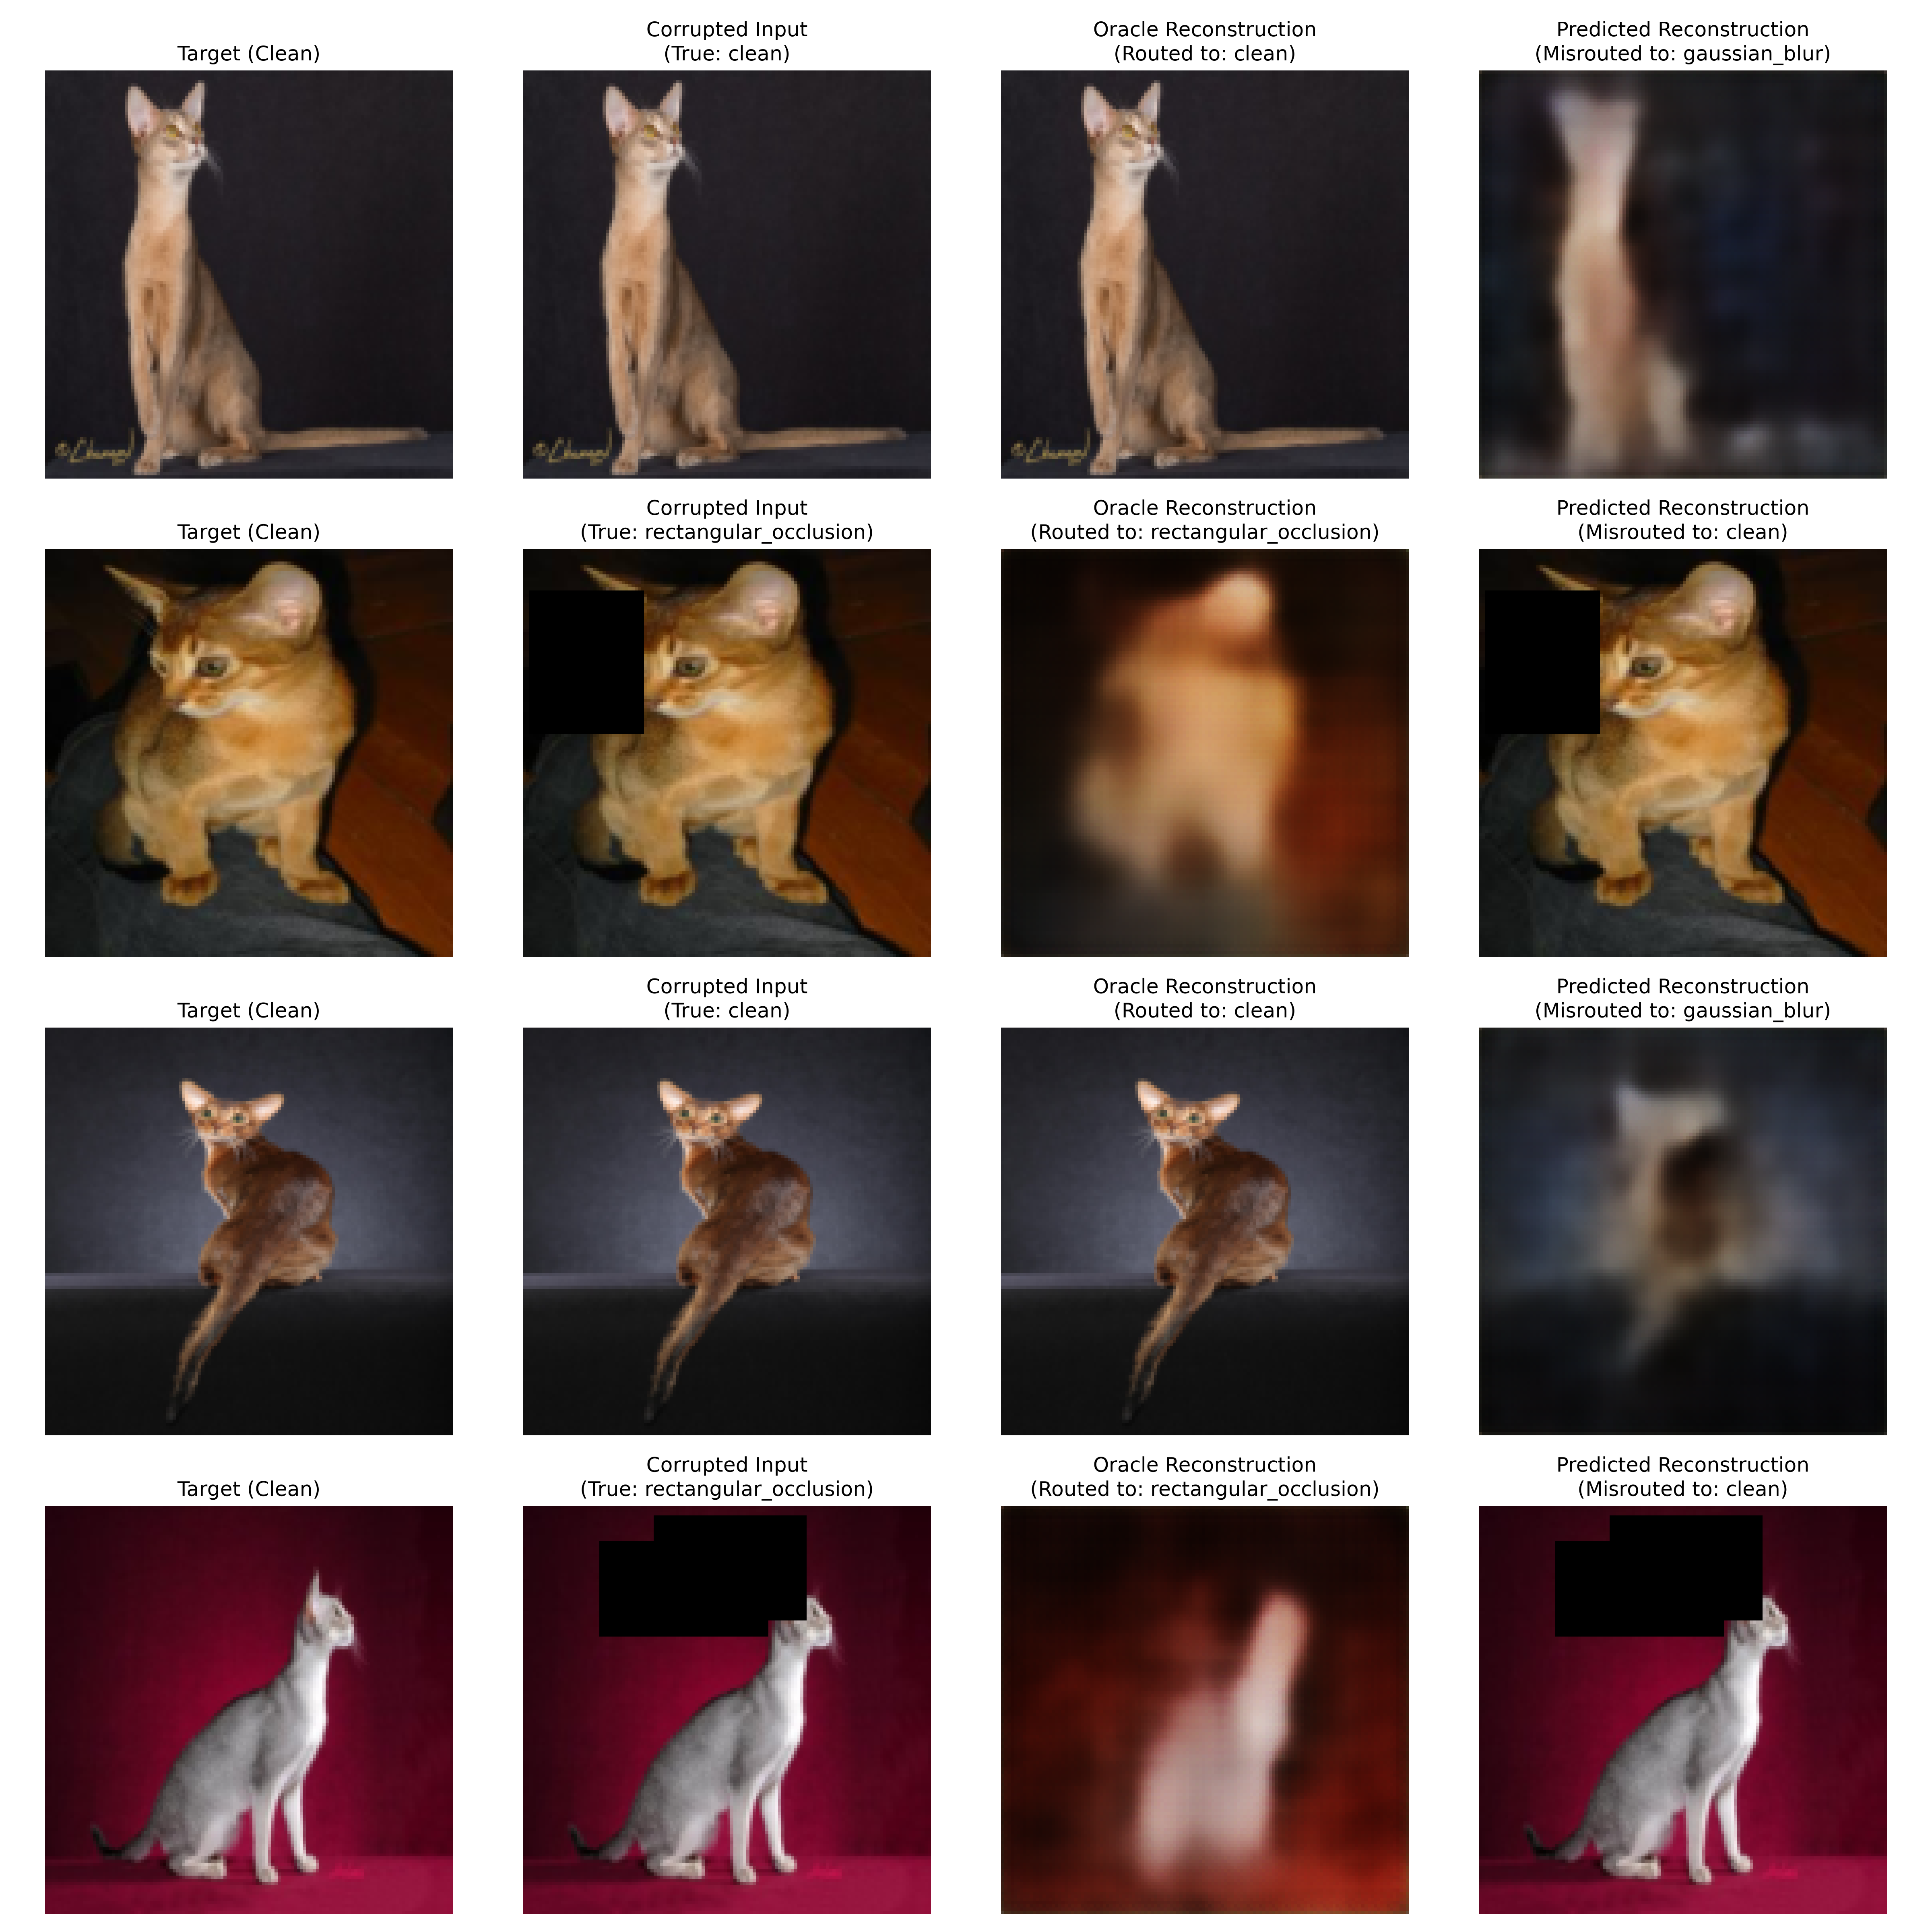
\includegraphics[width=\columnwidth]{task2/routing_failures.png}
\caption{Task 2: Cases where classifier misrouting produces visibly different outputs compared to oracle routing.}
\label{fig:task2_failures}
\end{figure}

% ============================================================
\section{Task 3: Jointly Trained Soft Mixture-of-Experts Restoration}
\label{sec:task3}

\subsection{Architecture}

\begin{figure}[H]
\centering
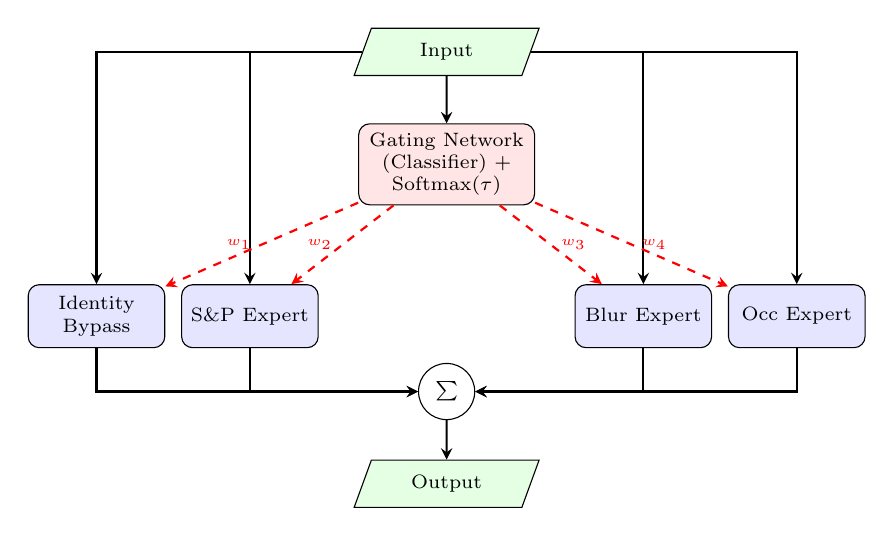
\begin{tikzpicture}[
    node distance=0.5cm and 0.3cm,
    expert/.style={rectangle, draw, fill=blue!10, text width=1.5cm, text centered, rounded corners, minimum height=0.8cm, font=\scriptsize},
    gate/.style={rectangle, draw, fill=red!10, text width=2cm, text centered, rounded corners, minimum height=0.8cm, font=\scriptsize},
    io/.style={trapezium, trapezium left angle=70, trapezium right angle=110, draw, fill=green!10, text width=1.2cm, text centered, minimum height=0.6cm, font=\scriptsize},
    arrow/.style={thick,->,>=stealth}
]
    \node [io] (input) {Input};
    
    \node [gate, below=0.6cm of input] (gating) {Gating Network (Classifier) + Softmax($\tau$)};
    
    \node [expert, below left=1cm and 0.5cm of gating] (exp2) {S\&P Expert};
    \node [expert, left=0.2cm of exp2] (exp1) {Identity Bypass};
    \node [expert, below right=1cm and 0.5cm of gating] (exp3) {Blur Expert};
    \node [expert, right=0.2cm of exp3] (exp4) {Occ Expert};
    
    \node [circle, draw, below=2cm of gating, font=\scriptsize] (sum) {$\sum$};
    \node [io, below=0.5cm of sum] (output) {Output};

    \draw [arrow] (input) -- (gating);
    \draw [arrow] (input) -| (exp1);
    \draw [arrow] (input) -| (exp2);
    \draw [arrow] (input) -| (exp3);
    \draw [arrow] (input) -| (exp4);
    
    \draw [arrow, dashed, red] (gating) -- (exp1) node[midway, left, font=\tiny] {$w_1$};
    \draw [arrow, dashed, red] (gating) -- (exp2) node[midway, left, font=\tiny] {$w_2$};
    \draw [arrow, dashed, red] (gating) -- (exp3) node[midway, right, font=\tiny] {$w_3$};
    \draw [arrow, dashed, red] (gating) -- (exp4) node[midway, right, font=\tiny] {$w_4$};
    
    \draw [arrow] (exp1) |- (sum);
    \draw [arrow] (exp2) |- (sum);
    \draw [arrow] (exp3) |- (sum);
    \draw [arrow] (exp4) |- (sum);
    
    \draw [arrow] (sum) -- (output);
\end{tikzpicture}
\caption{Task 3: Soft Mixture-of-Experts Architecture.}
\label{fig:arch_task3}
\end{figure}

The soft MoE model contains four branches: an identity pathway for clean images and three specialist autoencoders (initialized from Task~2). A gating network (initialized from the Task~2 classifier) computes continuous routing weights via temperature-scaled softmax:
\begin{equation}
w = \text{softmax}\left(\frac{G(x_c)}{\tau}\right)
\end{equation}
where $\tau$ is a non-learnable temperature parameter tuned by Optuna. The final reconstruction is:
\begin{equation}
\hat{x} = w_1 x_c + w_2 A_{\text{sp}}(x_c) + w_3 A_{\text{blur}}(x_c) + w_4 A_{\text{occ}}(x_c)
\end{equation}

The temperature $\tau$ is registered as a buffer (not a learnable parameter) to prevent backpropagation from collapsing it to zero.

\subsection{Joint Loss Function}

\begin{equation}
\mathcal{L}_{\text{joint}} = \lambda_1 \mathcal{L}_{\text{L1}} + \lambda_2 (1 - \text{SSIM}) + \lambda_3 \mathcal{L}_{\text{CE}} + \lambda_4 \mathcal{L}_{\text{balance}}
\end{equation}

The balance regularizer prevents routing collapse by penalizing deviation from uniform distribution:
\begin{equation}
\mathcal{L}_{\text{balance}} = \sum_{k=1}^{4}\left(\bar{w}_k - \frac{1}{4}\right)^2
\end{equation}
where $\bar{w}_k$ is the mean routing weight for branch $k$ within a batch. The cross-entropy component keeps the gating weights semantically aligned with the known corruption labels.

\subsection{Two-Stage Training}

\textbf{Stage 1 — Warm-up (10 epochs):} Expert parameters are frozen; only the gating network is trained using a dedicated warm-up learning rate. This prevents chaotic gradients from the untrained gate from destroying the pre-trained specialist weights.

\textbf{Stage 2 — Joint Fine-tuning ($\leq$100 epochs):} All parameters are unfrozen and trained jointly with a smaller fine-tuning learning rate. Early stopping with patience~5 and $\delta = 0.0005$ monitors the validation reconstruction loss.

\subsection{Hyperparameter Optimization}

\begin{table}[H]
\centering
\caption{Task 3 MoE: Optuna Search Space}
\label{tab:task3_hpo}
\begin{tabular}{lc}
\toprule
\textbf{Parameter} & \textbf{Search Range} \\
\midrule
Warm-up LR & $[10^{-5}, 10^{-3}]$ (log) \\
Fine-tune LR & $[10^{-6}, 10^{-4}]$ (log) \\
Temperature ($\tau$) & $[0.1, 5.0]$ \\
$\lambda_{\text{CE}}$ & $[0.01, 0.5]$ \\
$\lambda_{\text{balance}}$ & $[10^{-3}, 0.1]$ (log) \\
$\lambda_{\text{recon}}$ & $[0.1, 1.0]$ \\
$\lambda_{\text{SSIM}}$ & $[0.1, 1.0]$ \\
\bottomrule
\end{tabular}
\end{table}

The L1 and SSIM weights are treated as independent variables rather than a convex combination, providing the necessary mathematical freedom to balance pixel accuracy against structural quality on their different numerical scales. Custom trial pruning immediately terminates trials exhibiting routing collapse ($\max(\bar{w}) > 0.90$ or $\min(\bar{w}) < 0.05$).

\subsection{Experimental Results}

\begin{table}[H]
\centering
\caption{Task 3: Global Test Set Metrics (N=36,690)}
\label{tab:task3_global}
\begin{tabular}{lc}
\toprule
\textbf{Metric} & \textbf{Value} \\
\midrule
L1 Loss & 0.05281 \\
SSIM & 0.70292 \\
Avg Inference Time & 0.14 ms/image \\
\bottomrule
\end{tabular}
\end{table}

\begin{table}[H]
\centering
\caption{Task 3: Per-Corruption Metrics}
\label{tab:task3_corruption}
\begin{tabular}{lccc}
\toprule
\textbf{Corruption} & \textbf{Count} & \textbf{L1 $\downarrow$} & \textbf{SSIM $\uparrow$} \\
\midrule
Clean & 3,669 & 0.00873 & 0.99043 \\
Salt \& Pepper & 11,007 & 0.06947 & 0.52070 \\
Gaussian Blur & 11,007 & 0.04000 & 0.74703 \\
Rect. Occlusion & 11,007 & 0.06364 & 0.74518 \\
\bottomrule
\end{tabular}
\end{table}

The soft MoE achieves significantly better performance than both the universal autoencoder (Task~1: L1 = 0.074 avg) and the hard-routed system (Task~2: L1 = 0.068), reducing the overall L1 to 0.053 and improving SSIM from $\sim$0.51 to 0.70. The clean image pathway achieves near-perfect reconstruction (SSIM = 0.990).

\subsection{Routing Weight Analysis}

\begin{table}[H]
\centering
\caption{Task 3: Average Routing Weights by Corruption Type and Severity}
\label{tab:task3_routing}
\resizebox{\columnwidth}{!}{
\begin{tabular}{lcccc}
\toprule
\textbf{Condition} & \textbf{Identity} & \textbf{S\&P} & \textbf{Blur} & \textbf{Occ} \\
\midrule
Clean & \textbf{0.872} & 0.007 & 0.038 & 0.083 \\
S\&P (low) & 0.093 & \textbf{0.753} & 0.099 & 0.055 \\
S\&P (medium) & 0.002 & \textbf{0.968} & 0.006 & 0.025 \\
S\&P (high) & 0.000 & \textbf{0.980} & 0.000 & 0.020 \\
Blur (low) & \textbf{0.658} & 0.004 & 0.318 & 0.020 \\
Blur (medium) & \textbf{0.567} & 0.005 & 0.412 & 0.016 \\
Blur (high) & \textbf{0.560} & 0.006 & 0.415 & 0.020 \\
Occ (low) & \textbf{0.760} & 0.010 & 0.017 & 0.213 \\
Occ (medium) & \textbf{0.607} & 0.011 & 0.010 & 0.372 \\
Occ (high) & 0.427 & 0.010 & 0.007 & \textbf{0.556} \\
\bottomrule
\end{tabular}
}
\end{table}

\textbf{Key Observations:}

\begin{enumerate}
    \item \textbf{Clean images} are routed predominantly to the identity branch ($w = 0.872$), confirming that the gate learns to bypass unnecessary processing.
    \item \textbf{Salt-and-pepper} routing sharpens dramatically with severity: the S\&P expert weight increases from 0.753 (low) to 0.980 (high).
    \item \textbf{Gaussian blur} exhibits identity dominance even at high severity ($w_{\text{identity}} = 0.560$), suggesting the gate learned that the identity branch contributes useful high-frequency content that the blur expert alone cannot reconstruct.
    \item \textbf{Occlusion} shows progressive transfer from identity (0.760 at low severity) to the occlusion expert (0.556 at high severity), demonstrating severity-adaptive routing.
    \item All four experts remain active throughout evaluation, passing the inactivity check ($> 5\%$ total routing volume).
\end{enumerate}

\begin{figure}[H]
\centering
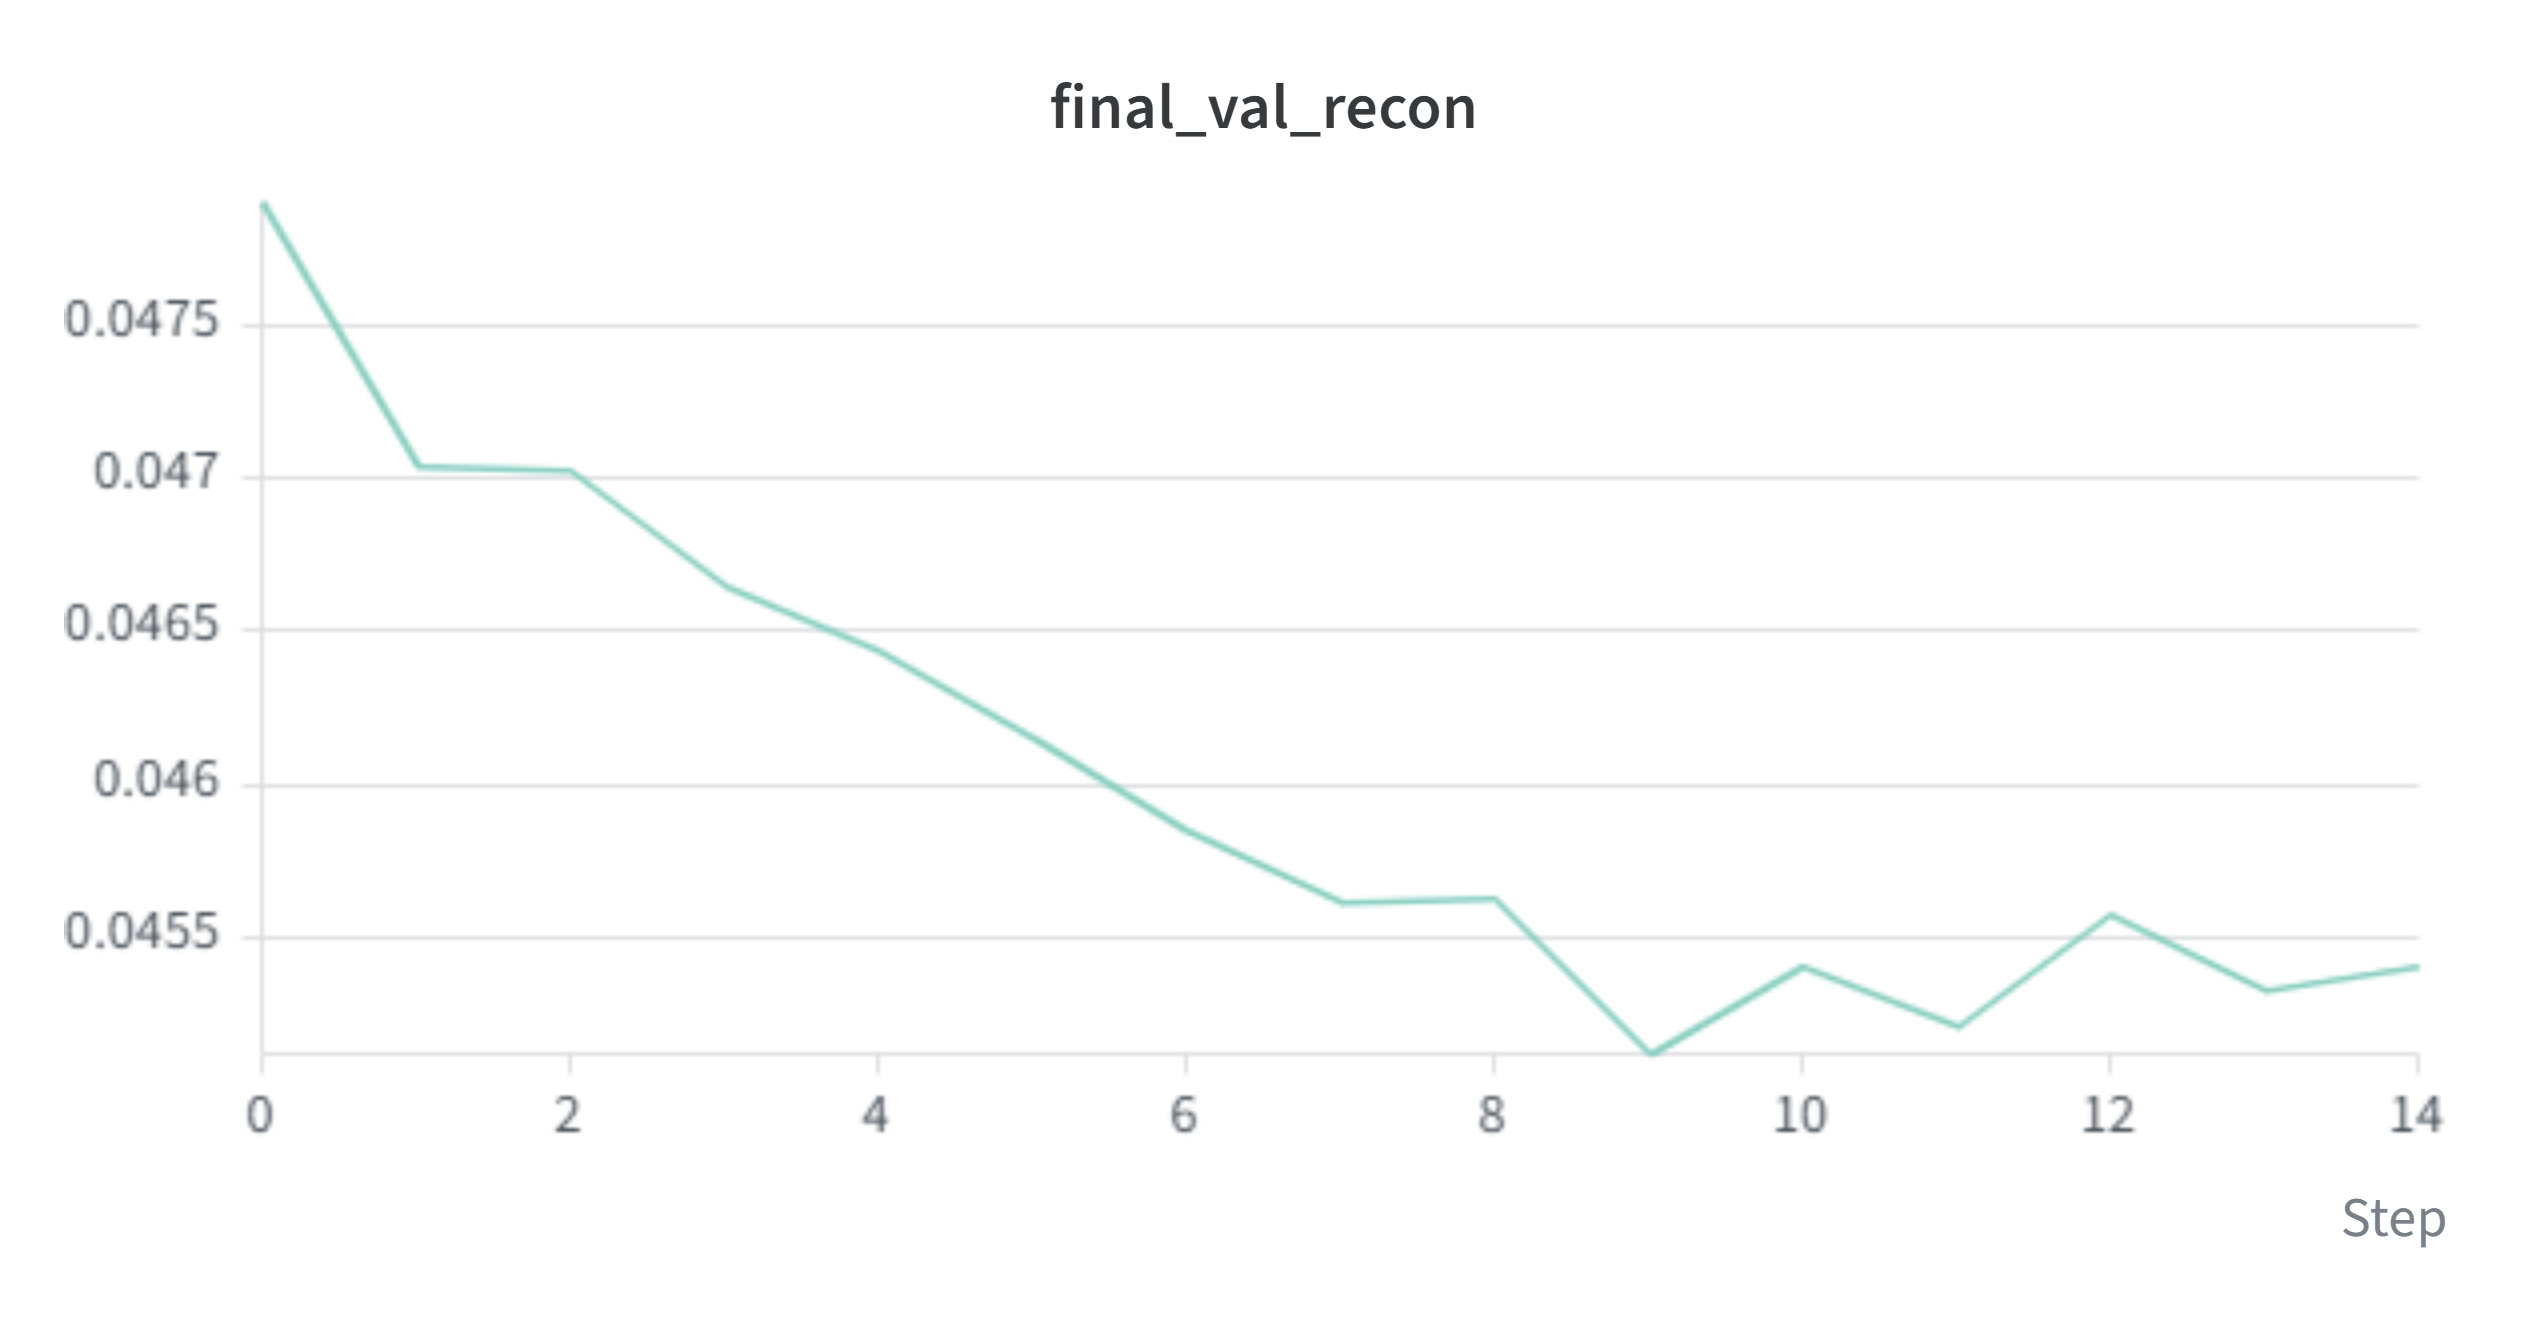
\includegraphics[width=0.7\columnwidth]{task3_val_recon_loss.png}
\caption{Task 3: Validation Reconstruction Loss vs Epoch during the joint fine-tuning stage. The loss descends smoothly and plateaus, confirming stable joint expert training.}
\label{fig:task3_curves}
\end{figure}

\begin{figure}[H]
\centering
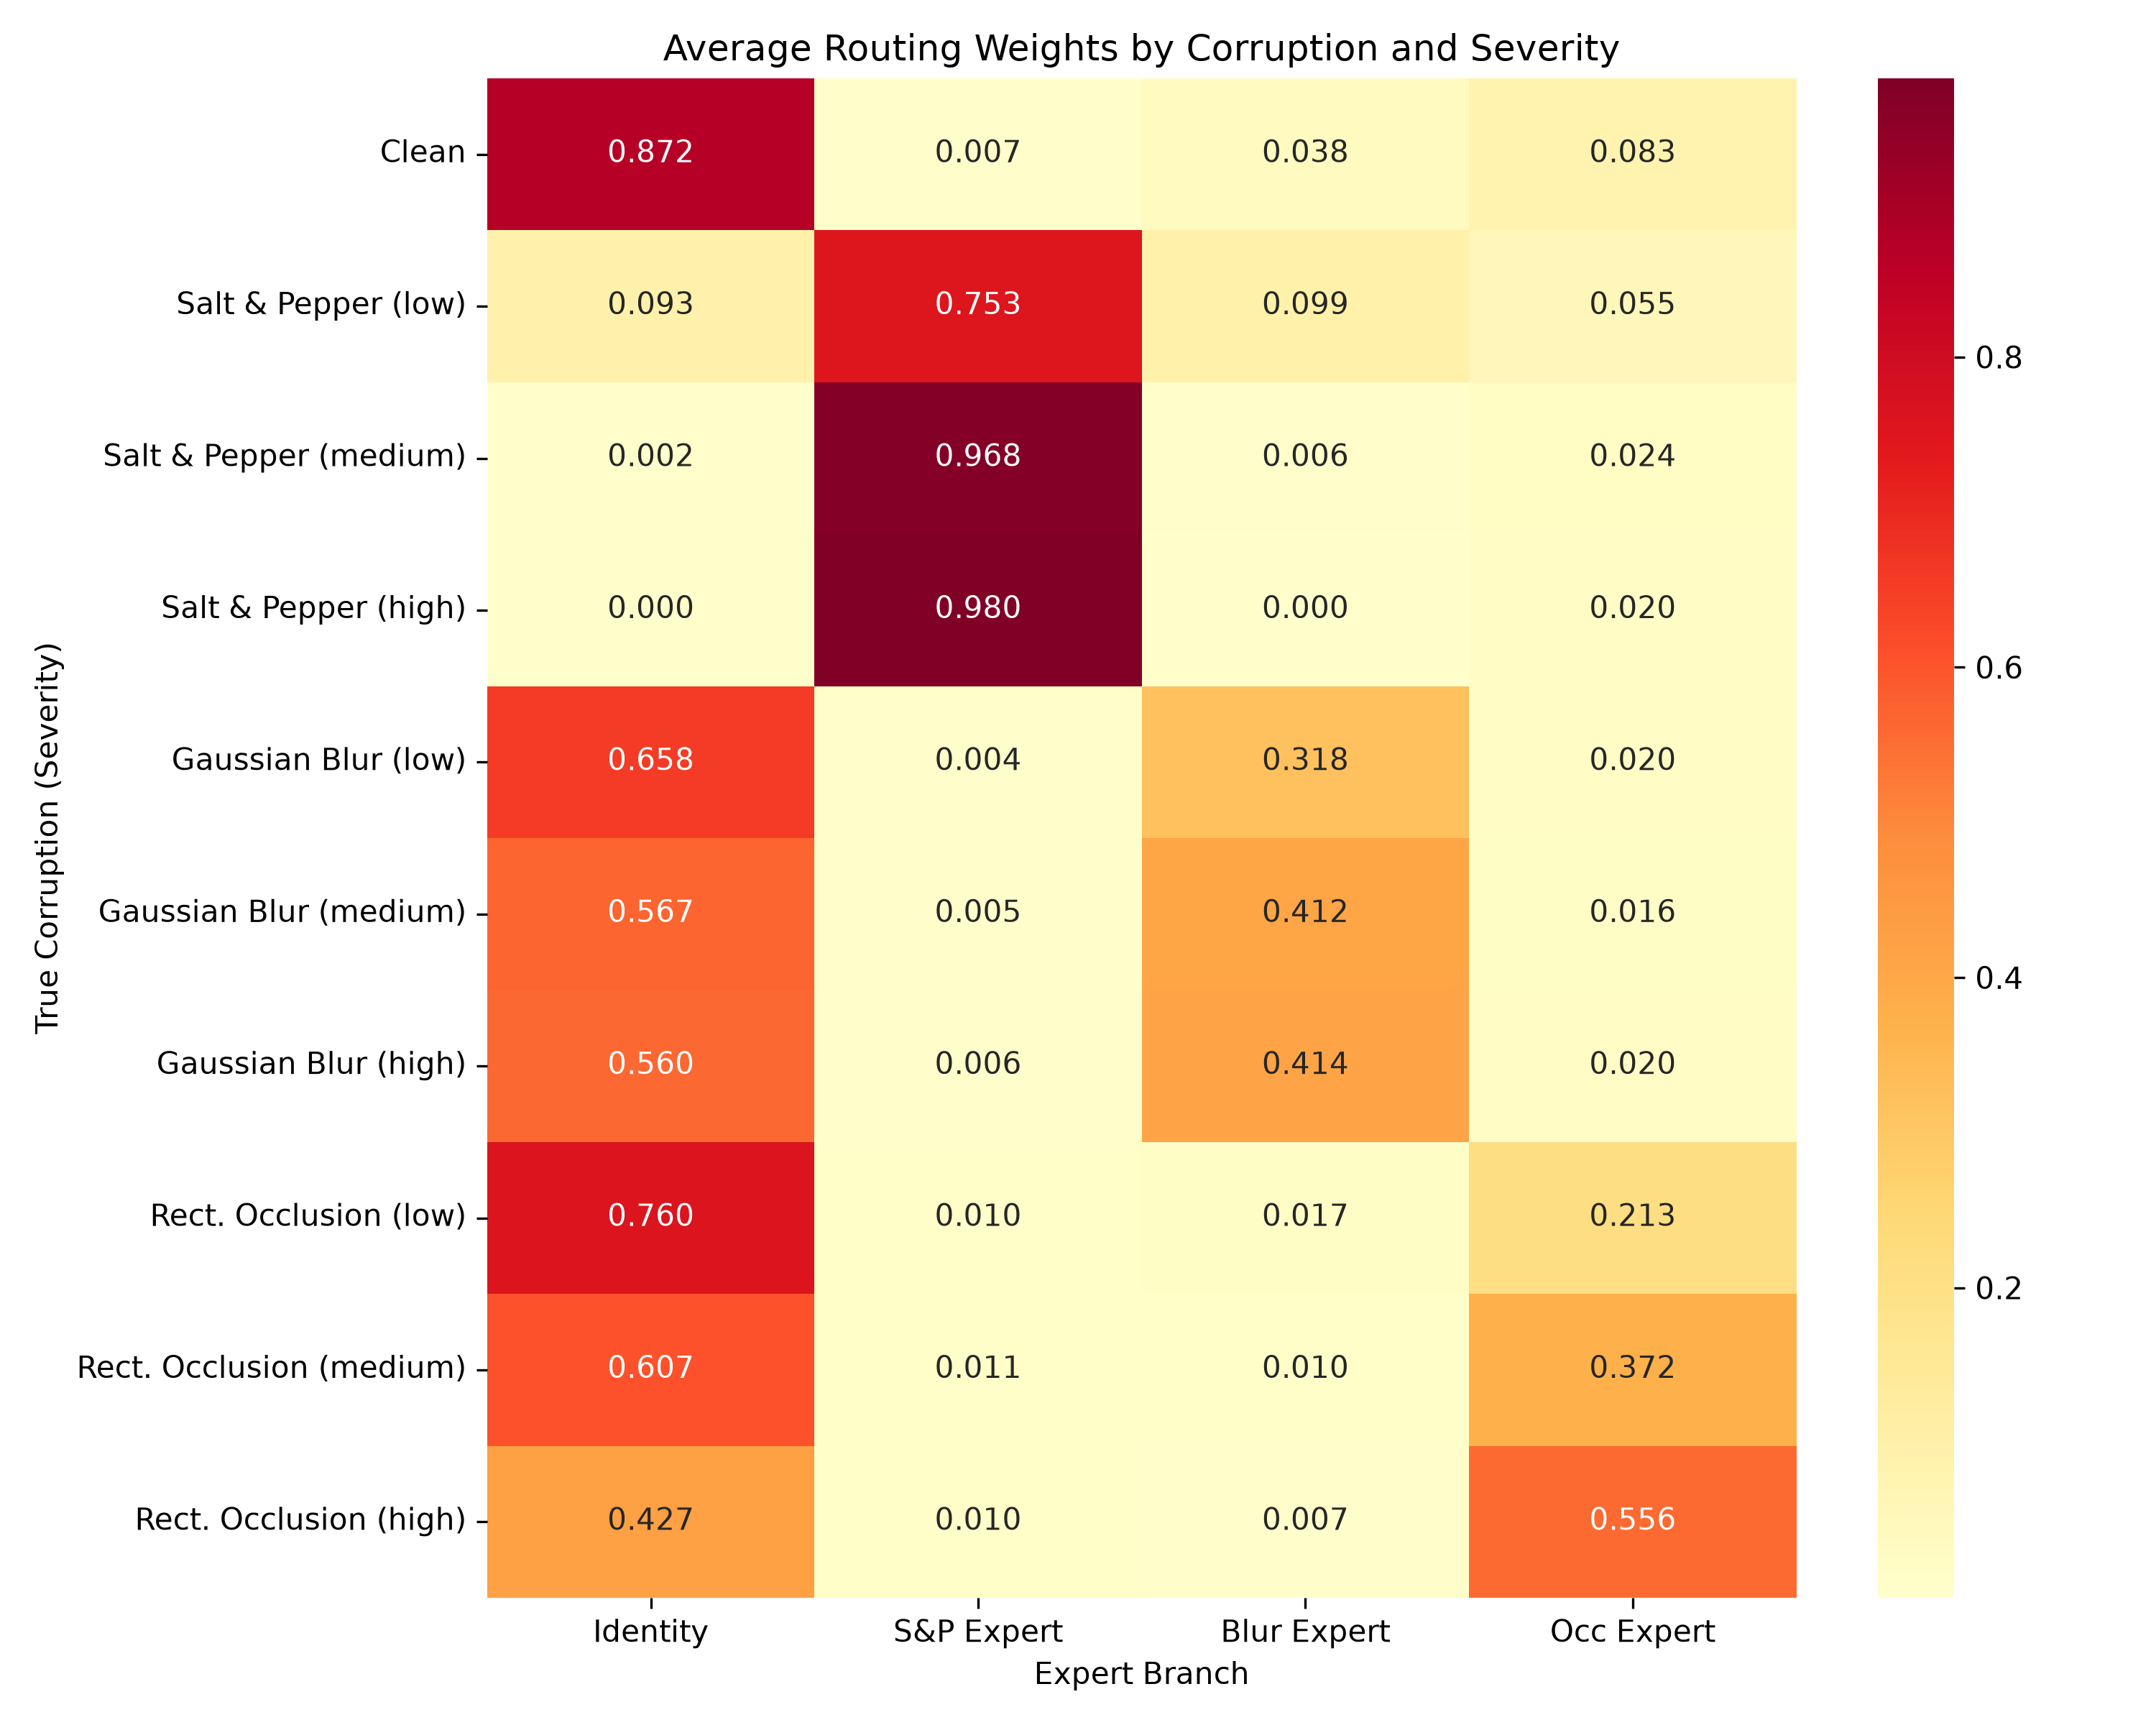
\includegraphics[width=0.85\columnwidth]{task3/routing_heatmap.png}
\caption{Task 3: Routing weight heatmap across corruption types and severity levels.}
\label{fig:task3_heatmap}
\end{figure}

\begin{figure}[H]
\centering
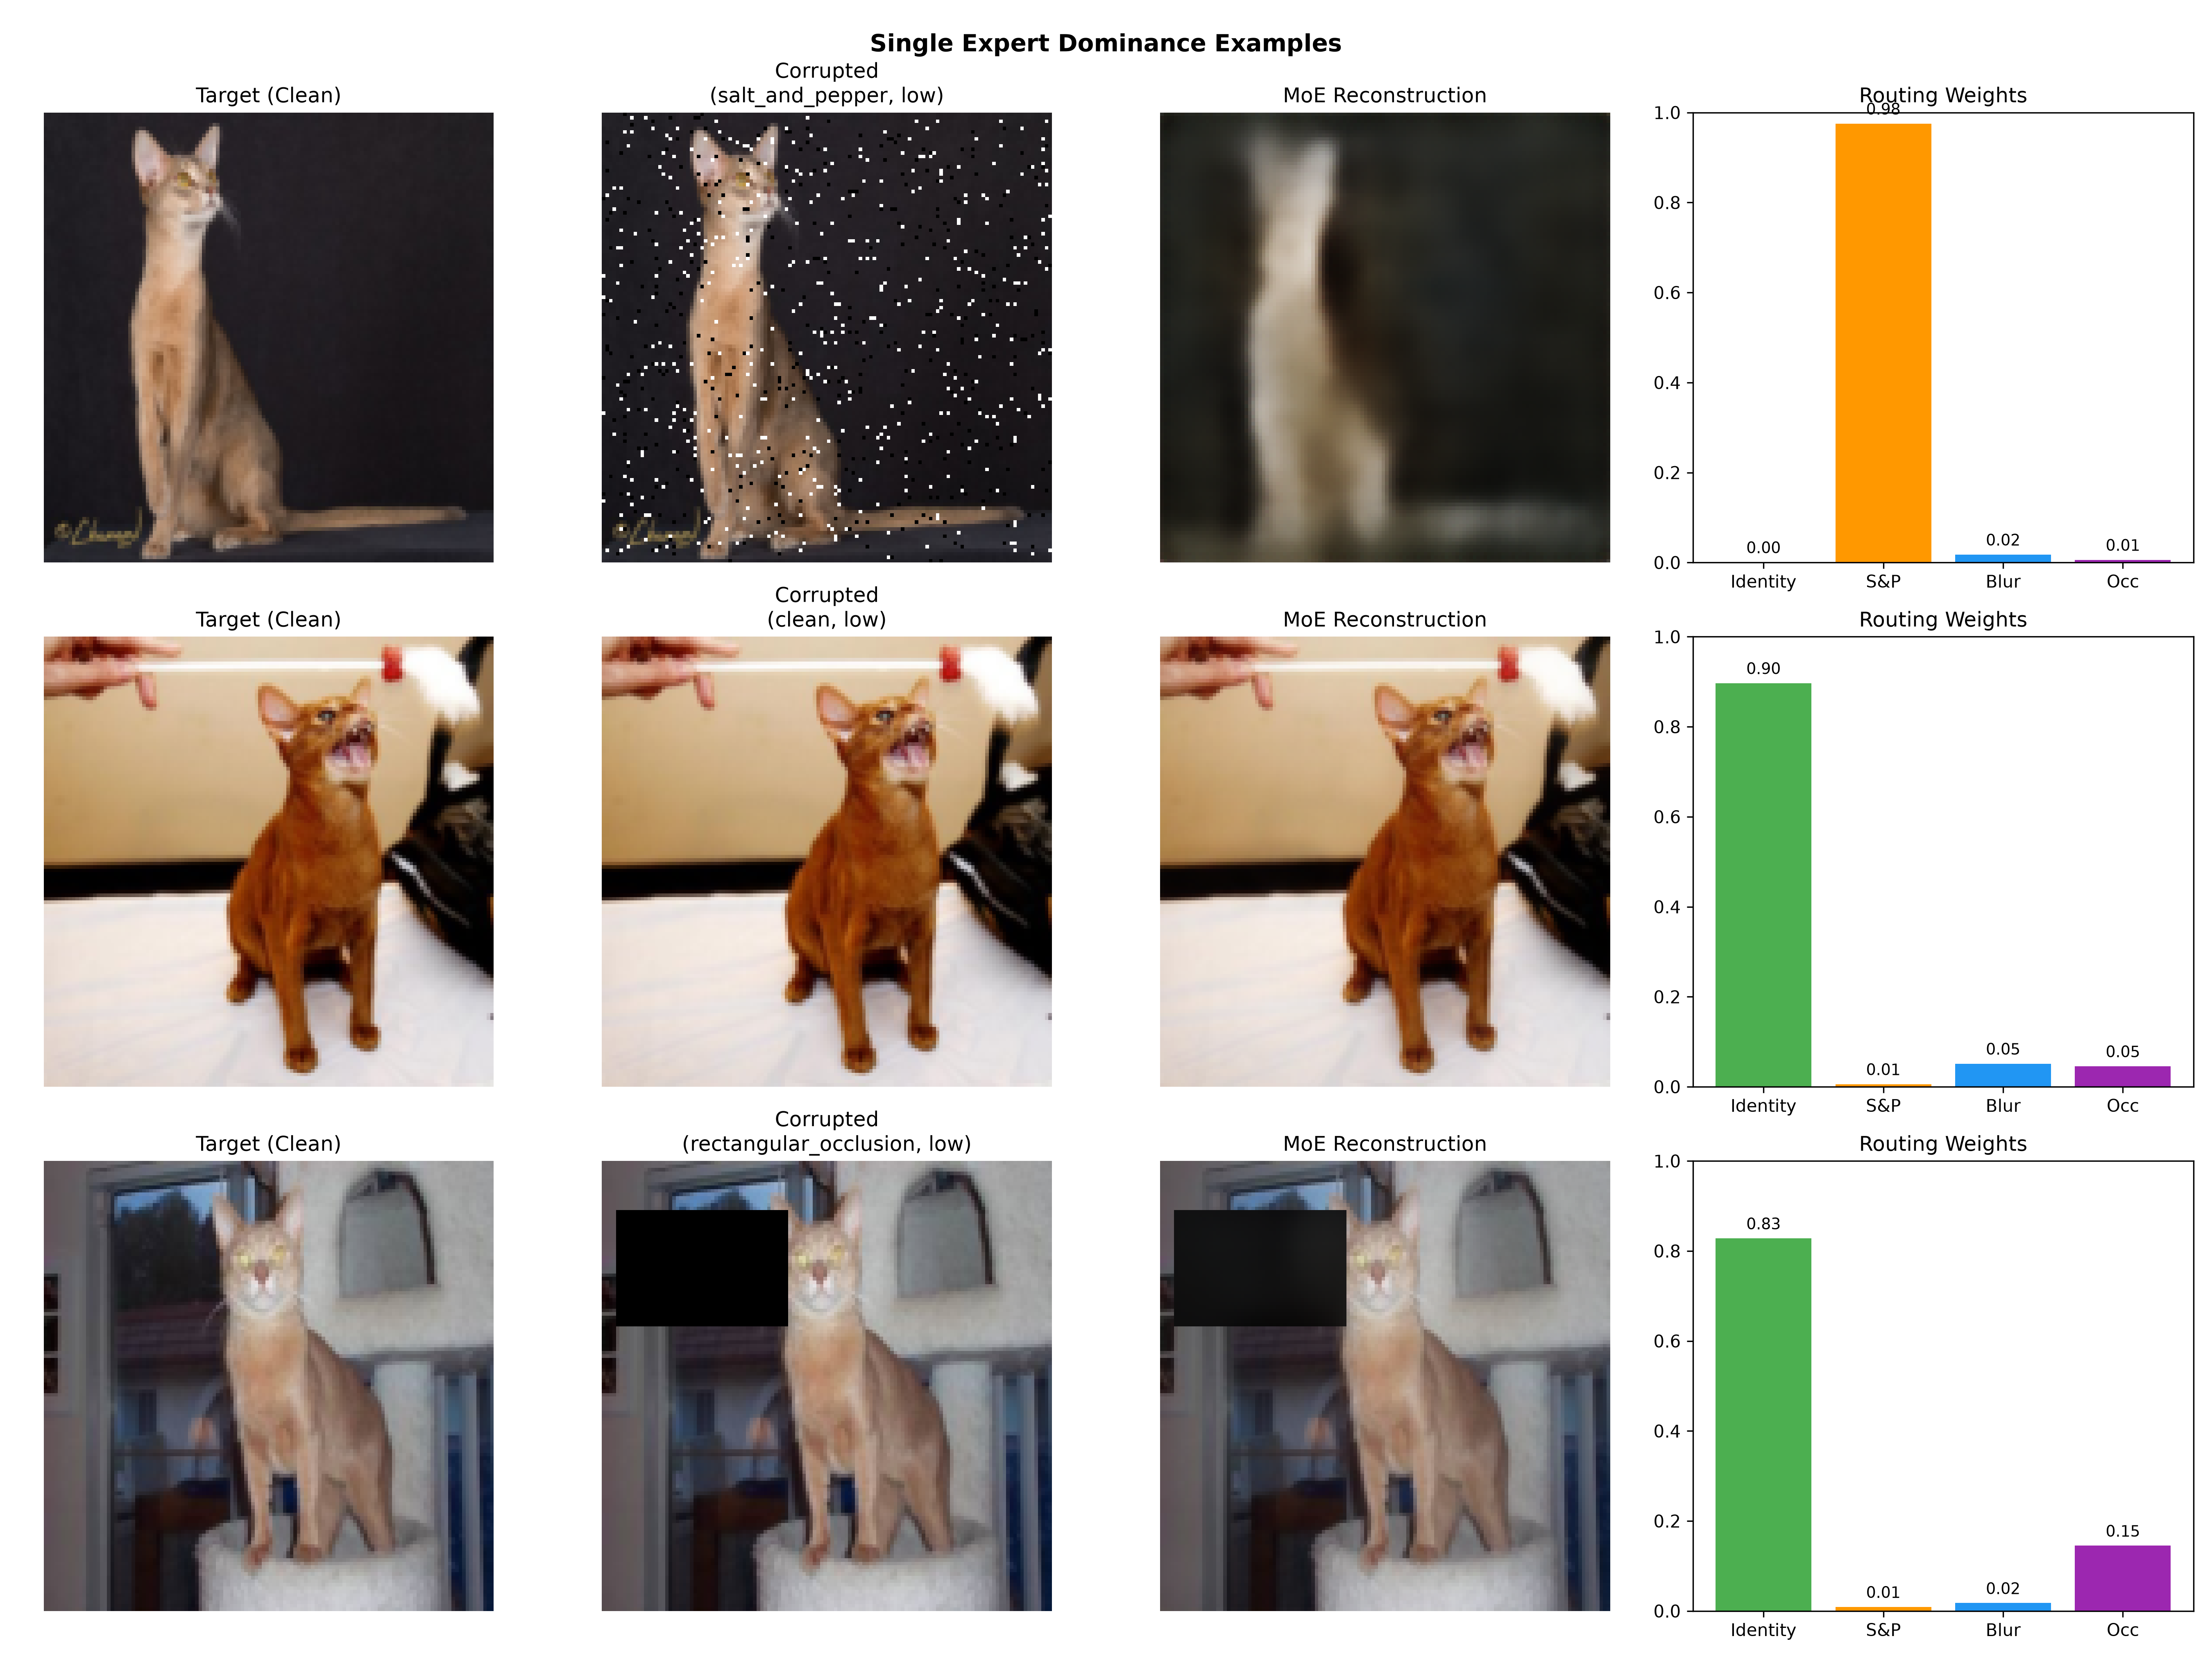
\includegraphics[width=\columnwidth]{task3/dominant_examples.png}
\caption{Task 3: Examples where a single expert dominates the routing weights.}
\label{fig:task3_dominant}
\end{figure}

\begin{figure}[H]
\centering
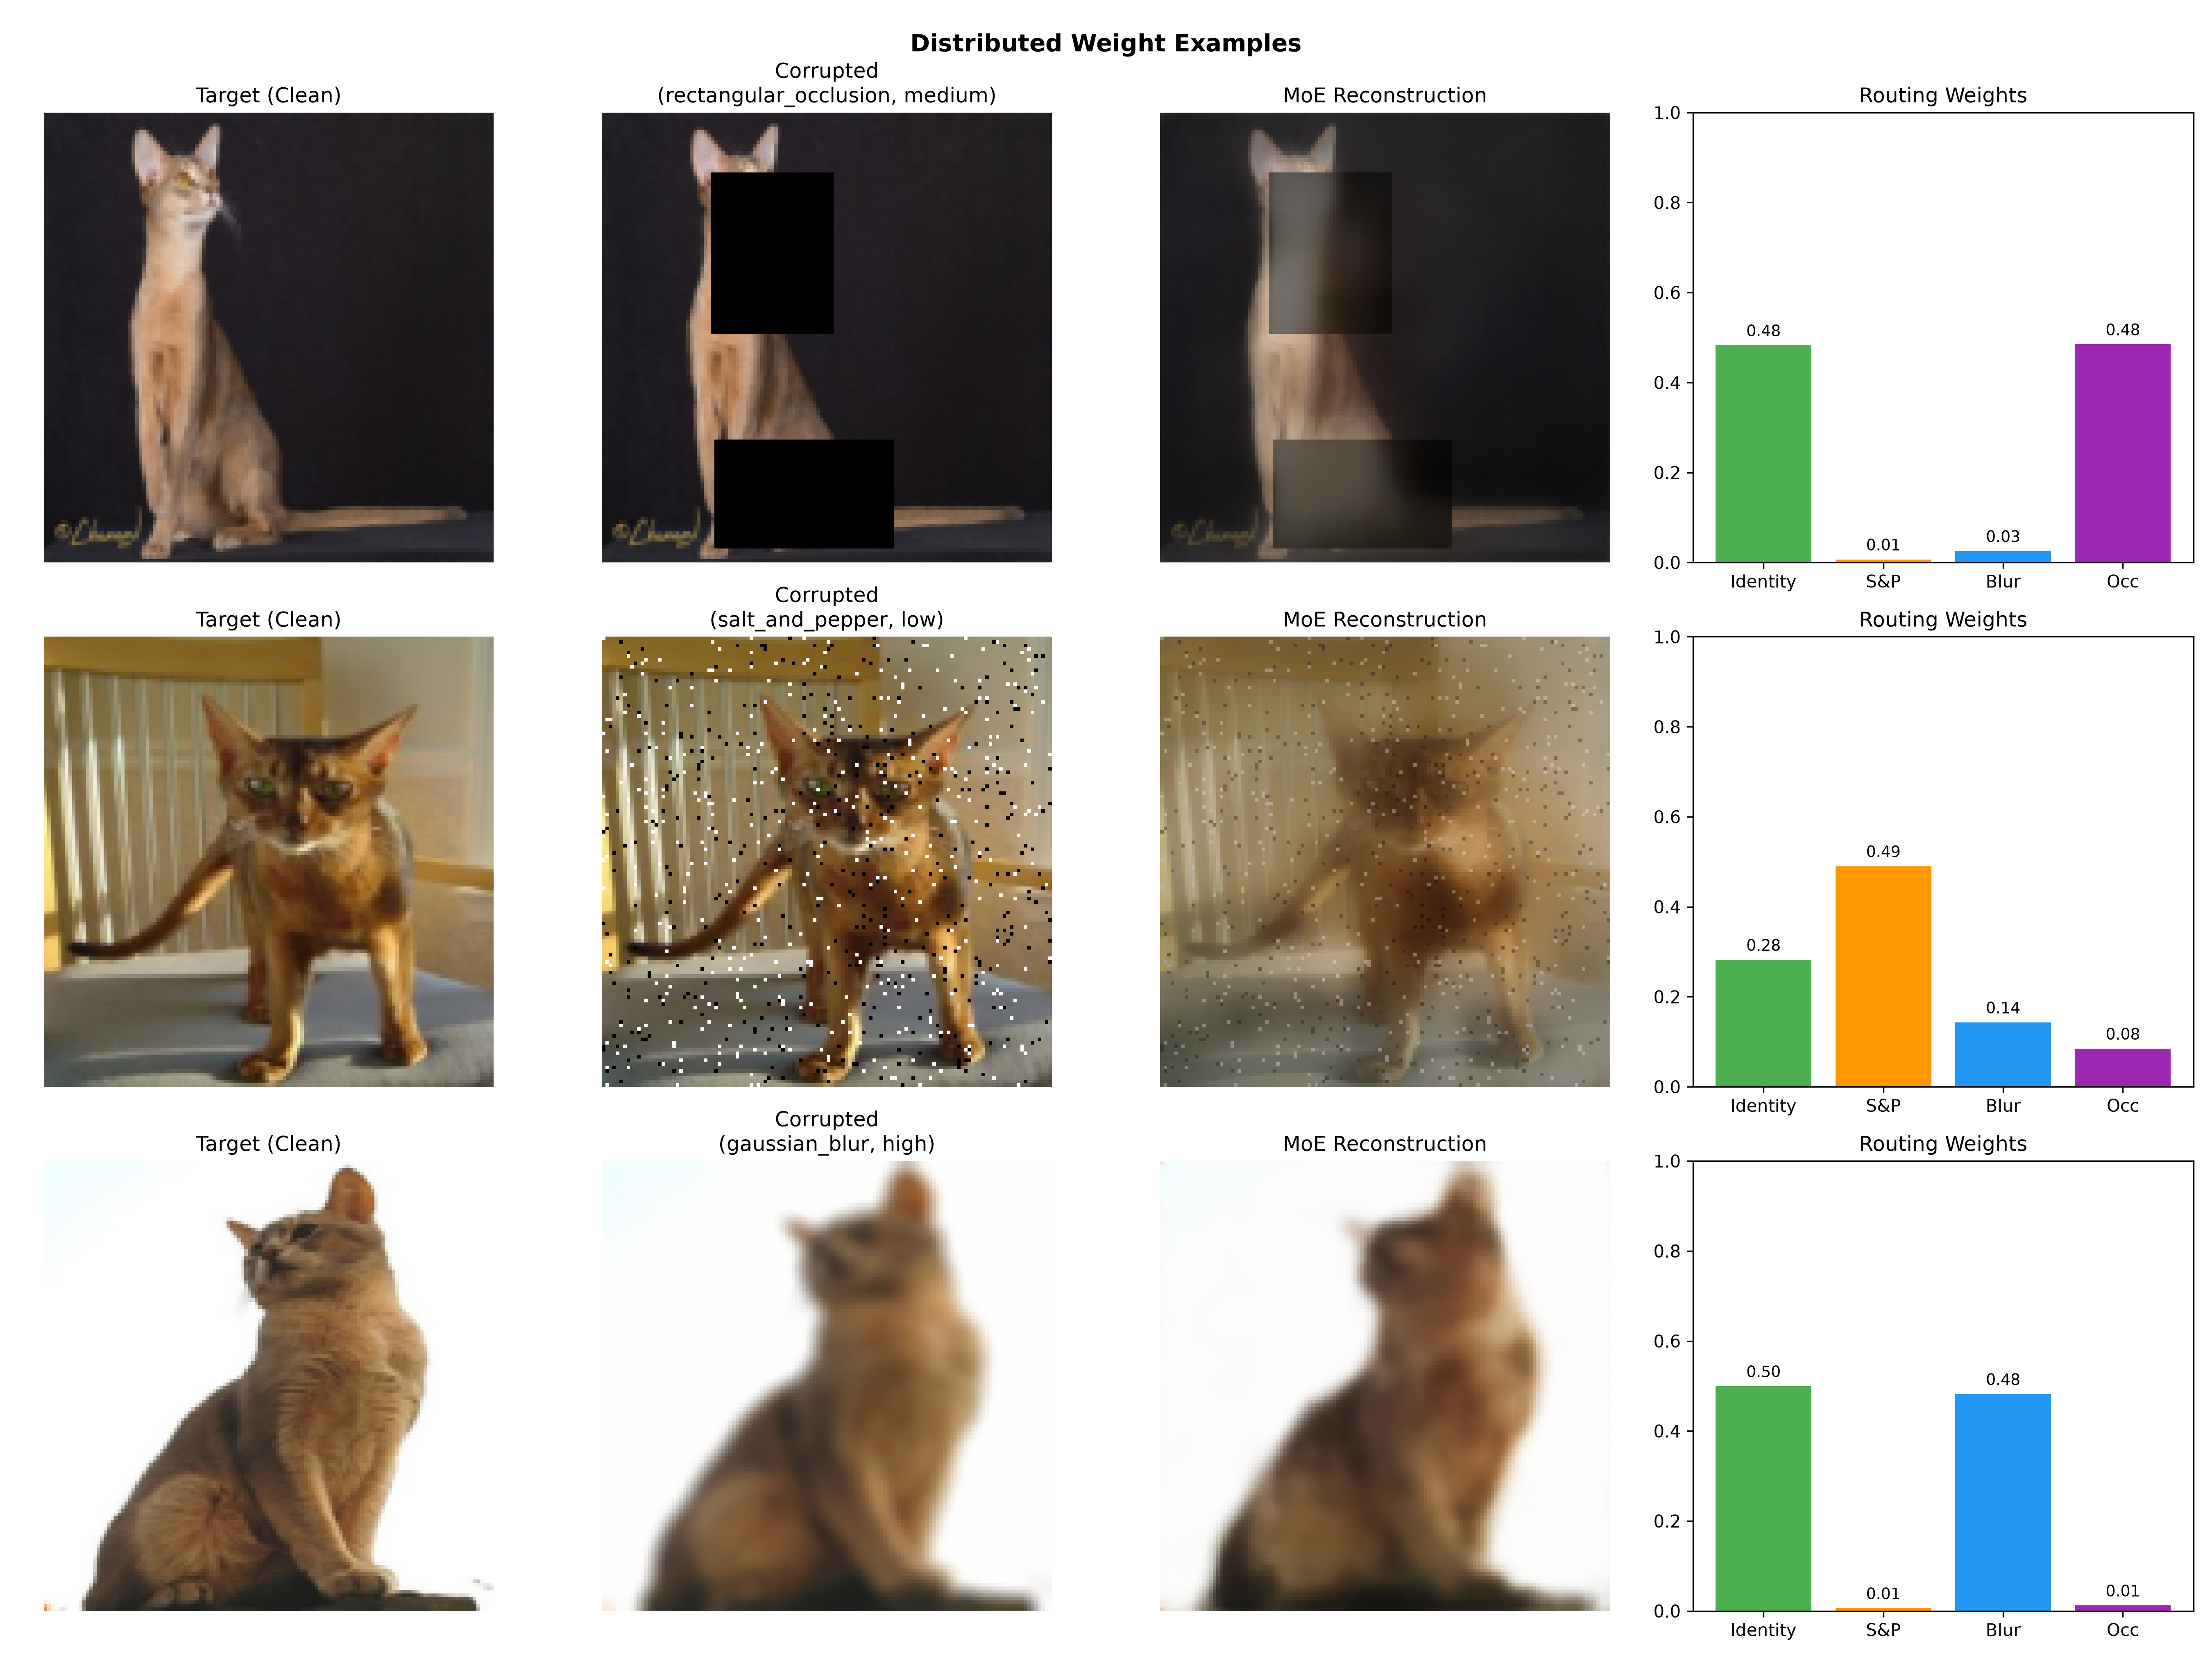
\includegraphics[width=\columnwidth]{task3/distributed_examples.png}
\caption{Task 3: Examples where routing weights are distributed across multiple experts.}
\label{fig:task3_distributed}
\end{figure}

% ============================================================
\section{Task 4: Style-Conditioned Face-to-Sketch Generation}
\label{sec:task4}

\subsection{Architecture}

\subsubsection{U-Net Generator}

\begin{figure}[H]
\centering
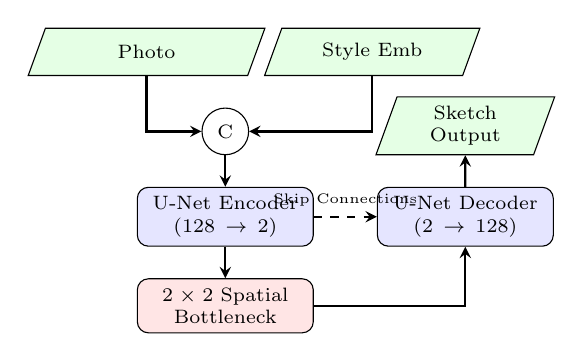
\begin{tikzpicture}[
    node distance=0.4cm and 0.4cm,
    block/.style={rectangle, draw, fill=blue!10, text width=2cm, text centered, rounded corners, minimum height=0.6cm, font=\scriptsize},
    io/.style={trapezium, trapezium left angle=70, trapezium right angle=110, draw, fill=green!10, text width=1.5cm, text centered, minimum height=0.6cm, font=\scriptsize},
    arrow/.style={thick,->,>=stealth}
]
    \node [io] (input) {Photo};
    \node [io, right=0.2cm of input] (style) {Style Emb};
    
    \node [circle, draw, below=0.4cm of input, xshift=1cm, font=\scriptsize] (concat1) {C};
    \node [block, below=0.4cm of concat1] (enc) {U-Net Encoder ($128\to2$)};
    
    \node [block, fill=red!10, below=of enc] (bottleneck) {$2\times2$ Spatial Bottleneck};
    
    \node [block, right=0.8cm of enc] (dec) {U-Net Decoder ($2\to128$)};
    \node [io, above=0.4cm of dec] (output) {Sketch Output};

    \draw [arrow] (input) |- (concat1);
    \draw [arrow] (style) |- (concat1);
    \draw [arrow] (concat1) -- (enc);
    \draw [arrow] (enc) -- (bottleneck);
    \draw [arrow] (bottleneck) -| (dec);
    \draw [arrow] (dec) -- (output);
    
    \draw [arrow, dashed] (enc) -- (dec) node[midway, above, font=\tiny] {Skip Connections};
\end{tikzpicture}
\caption{Task 4: Conditional U-Net Generator Architecture.}
\label{fig:arch_task4}
\end{figure}

The generator follows a 6-layer U-Net encoder-decoder architecture with skip connections. The style condition is incorporated via a learned categorical embedding (\texttt{nn.Embedding(3, $d_e$)}) that is spatially expanded to $d_e \times 128 \times 128$ and concatenated to the input photograph along the channel dimension, forming a $(3 + d_e)$-channel input.

The encoder uses $4 \times 4$ strided convolutions ($128 \rightarrow 64 \rightarrow 32 \rightarrow 16 \rightarrow 8 \rightarrow 4 \rightarrow 2$) with BatchNorm and LeakyReLU($0.2$). The bottleneck retains a $2 \times 2$ spatial resolution rather than collapsing to $1 \times 1$, preserving geometrically meaningful spatial layout information.

The decoder uses $4 \times 4$ transposed convolutions with BatchNorm, dropout (in the first two layers for regularization), and ReLU activations. Skip connections from the corresponding encoder layers are concatenated along the channel dimension before each decoder block. The output layer uses Tanh to produce values in $[-1, 1]$.

\textbf{Design Justification.} Using a learned embedding rather than a raw integer avoids imposing an artificial ordinal relationship between styles. The Tanh activation provides zero-centered, symmetric outputs with stronger gradients than Sigmoid, mitigating vanishing gradient problems in deep adversarial networks~\cite{isola2017image}.

\subsubsection{PatchGAN Discriminator}
The discriminator receives the concatenation of the input photograph, the sketch (real or generated), and the spatially expanded style embedding, forming a $(3 + 3 + d_e)$-channel input. It applies 5 convolutional layers: three with stride~2 ($128 \rightarrow 64 \rightarrow 32 \rightarrow 16$) and two with stride~1 ($16 \rightarrow 15 \rightarrow 14$), producing a $14 \times 14$ grid of patch-level real/fake logits. This PatchGAN design evaluates local regions for realism rather than making a single global judgment.

\subsection{Training Procedure}

The generator objective combines adversarial and reconstruction losses:
\begin{equation}
\mathcal{L}_G = \mathcal{L}_{\text{BCE}} + \lambda_{\text{L1}} \cdot \mathcal{L}_{\text{L1}}(y, G(x, s))
\end{equation}

The discriminator is trained with standard binary cross-entropy:
\begin{equation}
\mathcal{L}_D = \frac{1}{2}\left[\mathcal{L}_{\text{BCE}}(D(x, y, s), 1) + \mathcal{L}_{\text{BCE}}(D(x, G(x,s), s), 0)\right]
\end{equation}

Both networks use Adam with $\beta = (0.5, 0.999)$. A linear learning rate decay schedule keeps the rate constant for the first 50 epochs and linearly decays to zero over the remaining 50 epochs, stabilizing the adversarial equilibrium. Weight initialization follows $\mathcal{N}(0, 0.02)$ as established by the original Pix2Pix implementation.

Training logs record discriminator real/fake losses, generator adversarial/reconstruction losses, and validation metrics separately. Visual samples are logged to W\&B every 5 epochs using a fixed validation batch.

\subsection{Hyperparameter Optimization}

\begin{table}[H]
\centering
\caption{Task 4 GAN: Optuna Search Space}
\label{tab:task4_hpo}
\begin{tabular}{lc}
\toprule
\textbf{Parameter} & \textbf{Search Range} \\
\midrule
Generator LR & $[10^{-5}, 10^{-3}]$ (log) \\
Discriminator LR & $[10^{-5}, 10^{-3}]$ (log) \\
Batch size & $\{8, 16, 32\}$ \\
Base channels & $\{32, 64, 128\}$ \\
Dropout & $[0.0, 0.5]$ \\
Embedding dim & $\{8, 16, 32, 64\}$ \\
$\lambda_{\text{L1}}$ & $[10.0, 200.0]$ \\
\bottomrule
\end{tabular}
\end{table}

HPO trials used 15 epochs each due to GAN training expense. The best configuration was then retrained for the full 100-epoch schedule.

\subsection{Experimental Results}

\begin{table}[H]
\centering
\caption{Task 4: Per-Style Test Set Metrics}
\label{tab:task4_results}
\begin{tabular}{lcccc}
\toprule
\textbf{Style} & \textbf{Count} & \textbf{L1 $\downarrow$} & \textbf{SSIM $\uparrow$} & \textbf{PSNR $\uparrow$} \\
\midrule
Style 0 & 619 & 0.0806 & 0.5358 & 17.10 \\
Style 1 & 381 & 0.1525 & 0.3926 & 12.42 \\
Style 2 & 46 & \textbf{0.0642} & \textbf{0.6371} & \textbf{18.61} \\
\bottomrule
\end{tabular}
\end{table}

Style~2 achieves the best reconstruction metrics despite having the fewest training examples, likely because its visual characteristics (line-drawing style) are most amenable to pixel-wise comparison. Style~1, which involves more complex artistic transformations, presents the greatest challenge. The final checkpoint (epoch~100) was exported rather than the best-validation checkpoint because GAN validation loss, heavily influenced by the adversarial BCE component, is an unreliable proxy for perceptual quality.

\begin{figure}[H]
\centering
\begin{subfigure}{0.48\columnwidth}
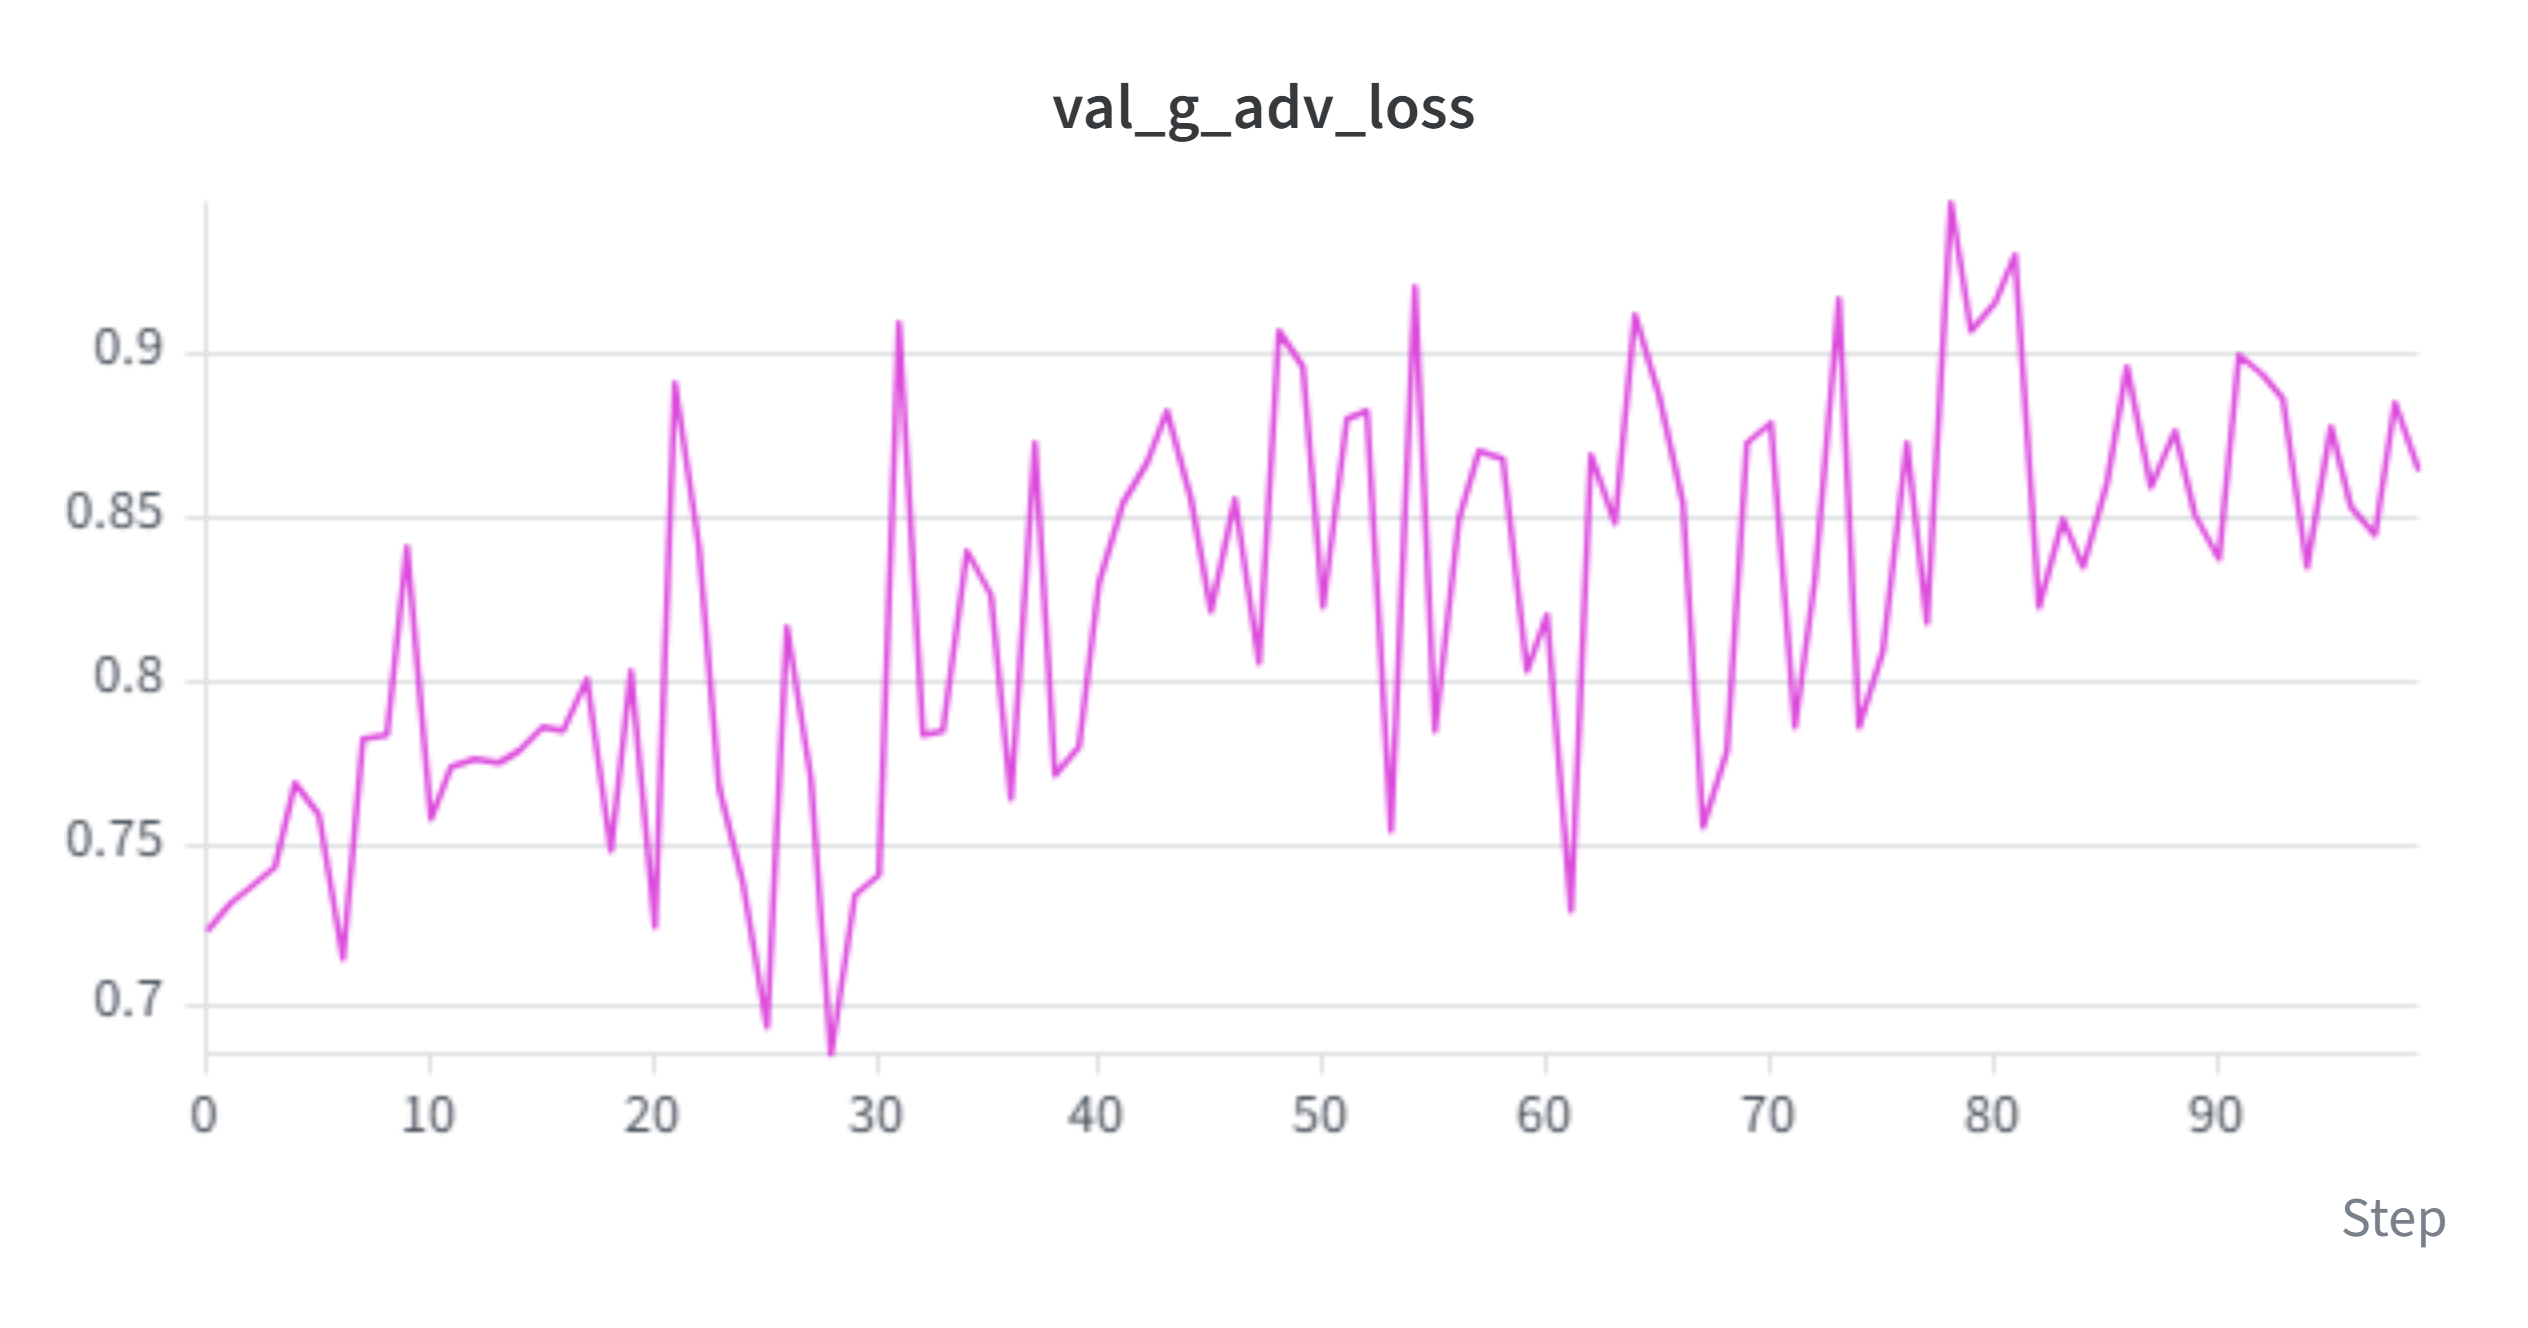
\includegraphics[width=\linewidth]{task4_val_gen_adv_loss.png}
\caption{Validation Adversarial Loss}
\end{subfigure}\hfill
\begin{subfigure}{0.48\columnwidth}
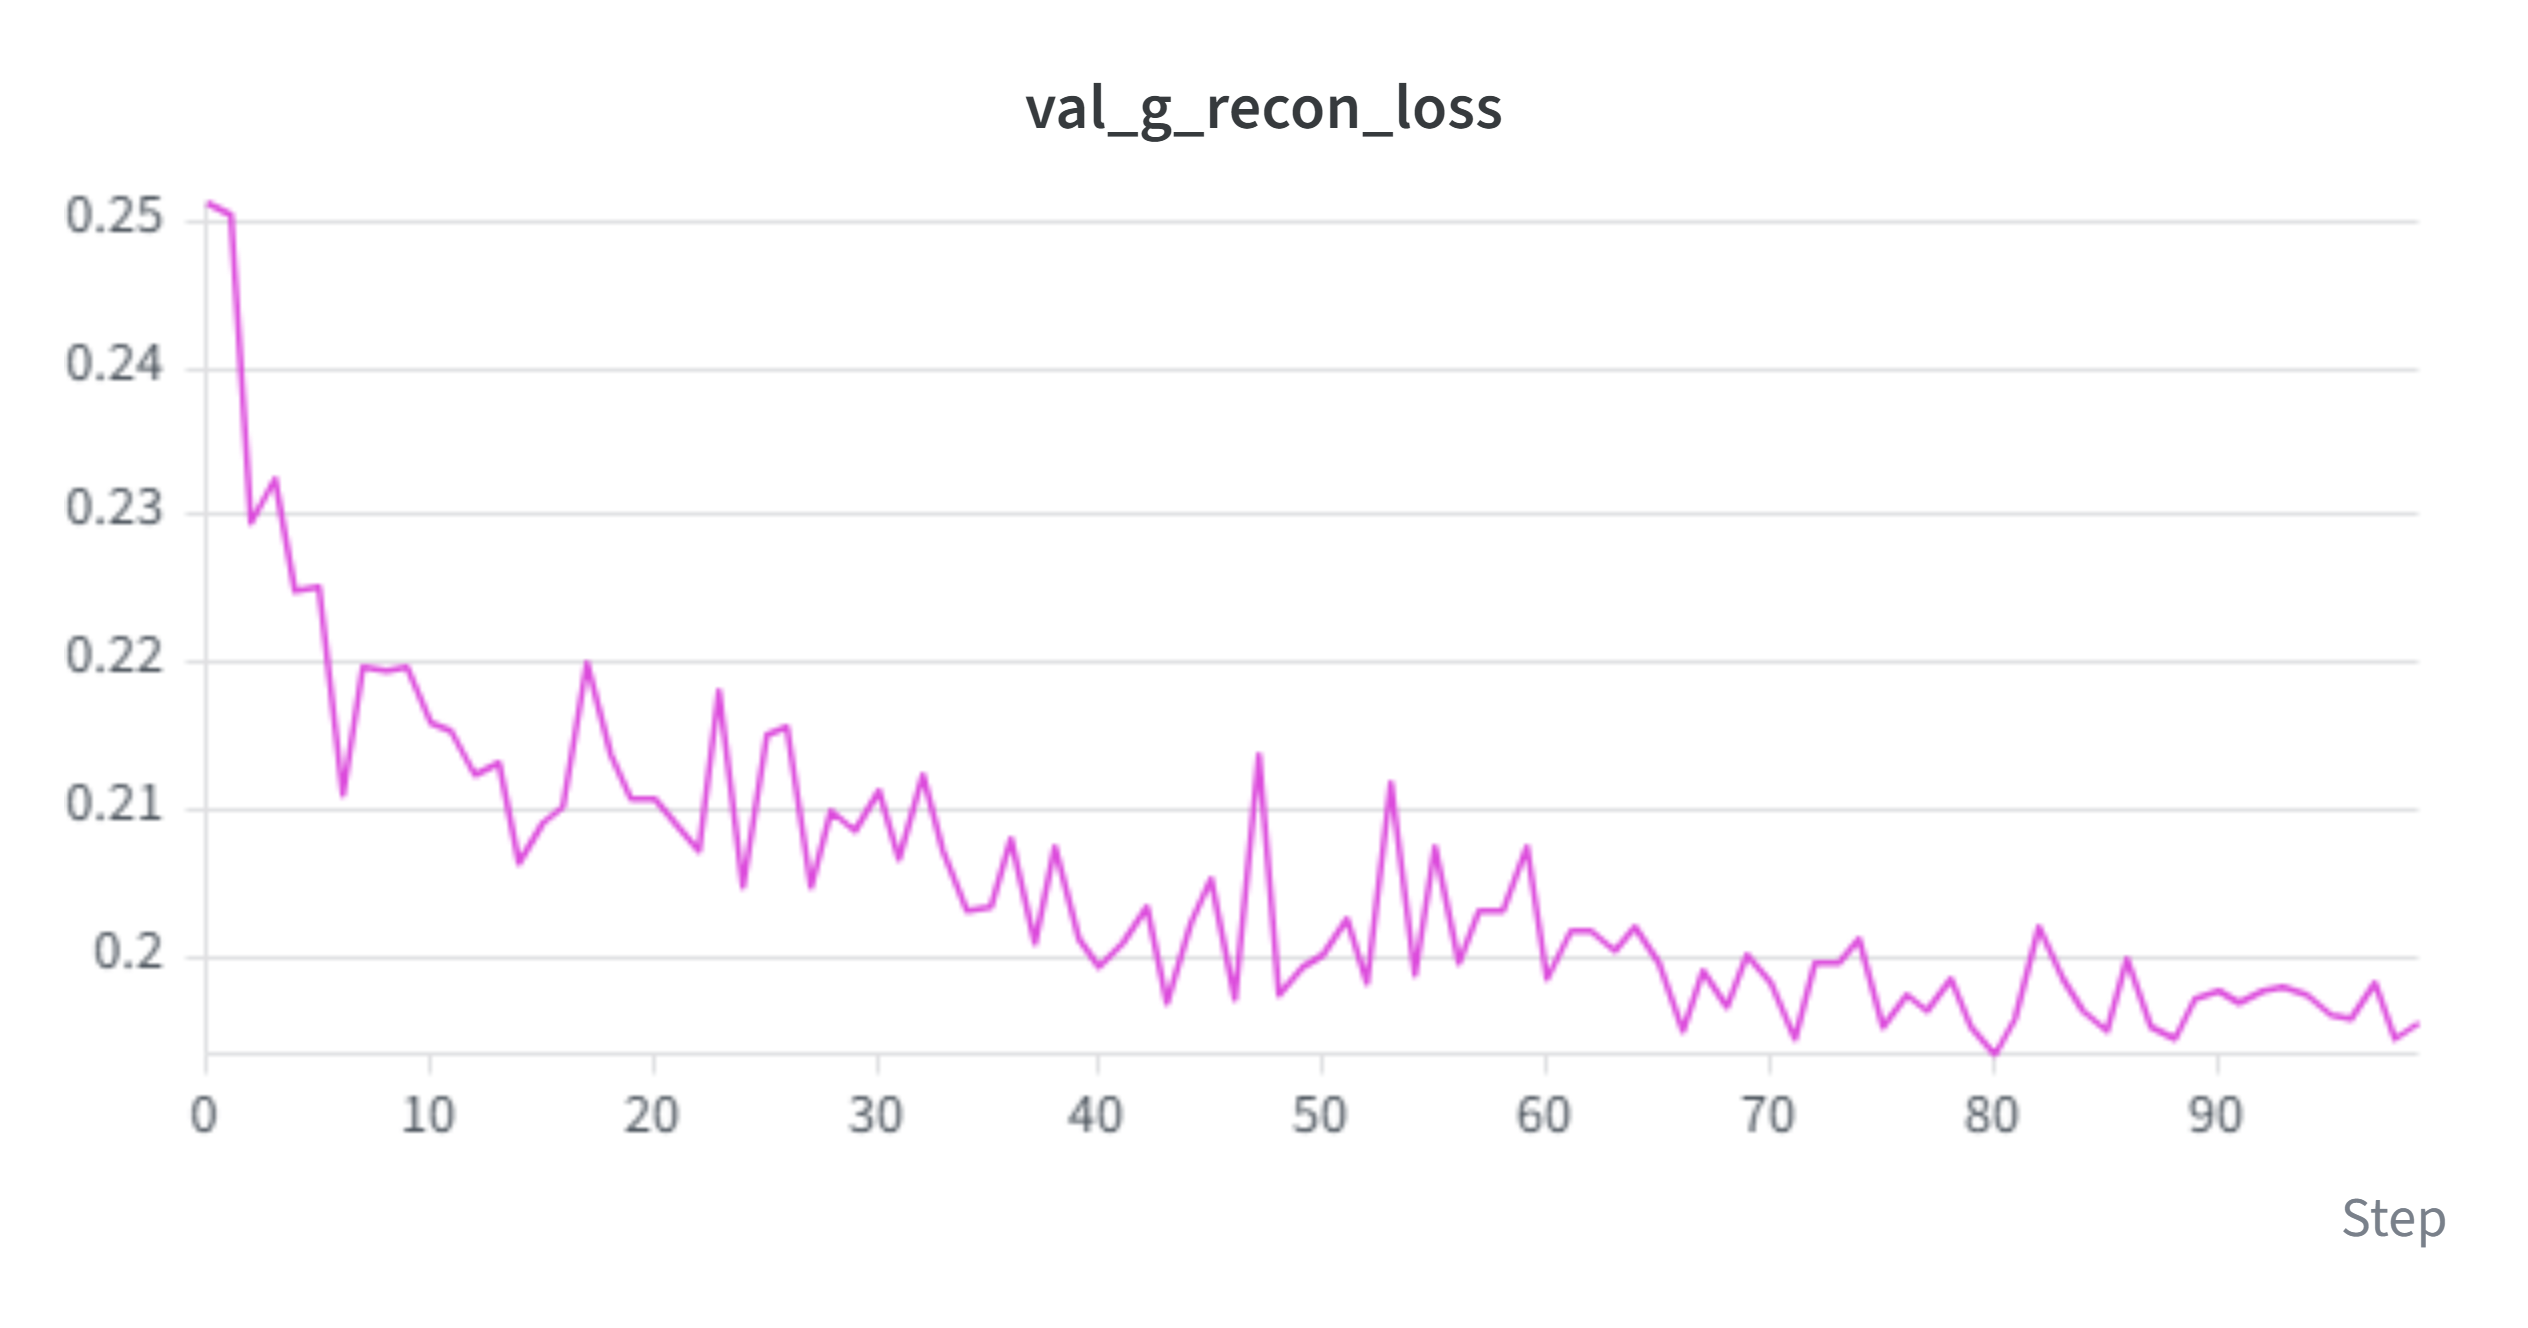
\includegraphics[width=\linewidth]{task4_val_gen_recon_loss.png}
\caption{Validation L1 Recon Loss}
\end{subfigure}
\caption{Task 4: Generator Validation Losses. The adversarial loss fluctuates as the discriminator and generator reach equilibrium, while L1 loss gradually decreases, ensuring structural fidelity.}
\label{fig:task4_curves}
\end{figure}

\begin{figure}[H]
\centering
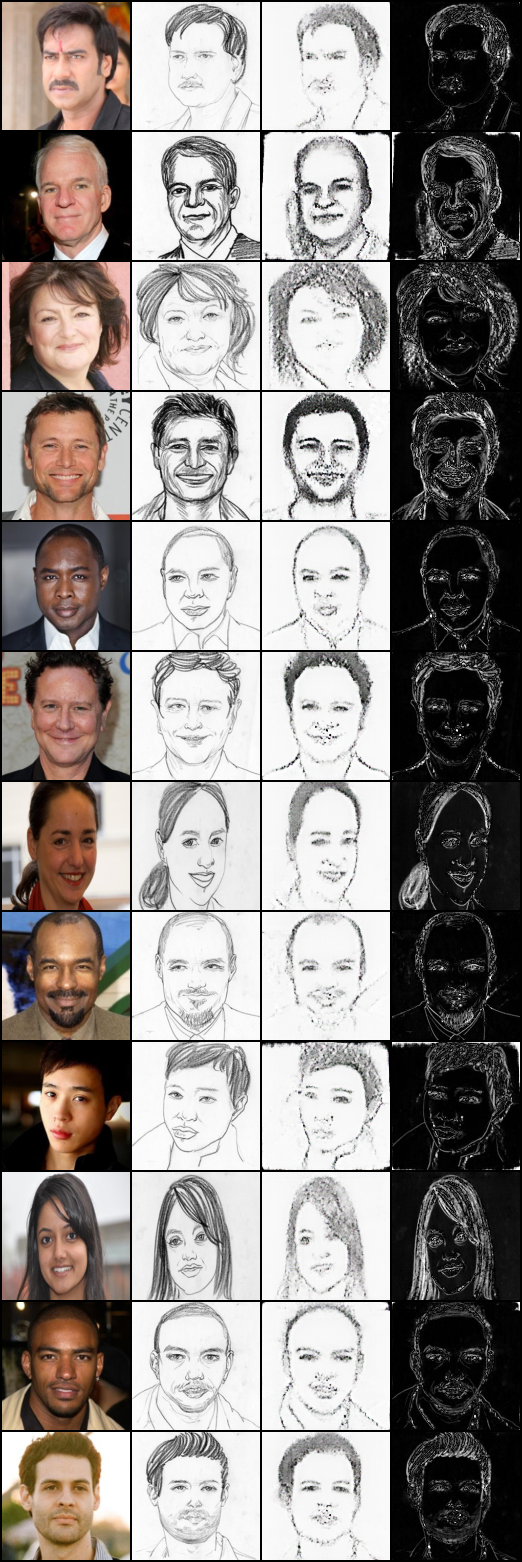
\includegraphics[width=\columnwidth]{task4/representative_examples.png}
\caption{Task 4: Representative face-to-sketch generation results. Columns: input photo, ground-truth sketch, generated sketch, L1 error map.}
\label{fig:task4_examples}
\end{figure}

\begin{figure}[H]
\centering
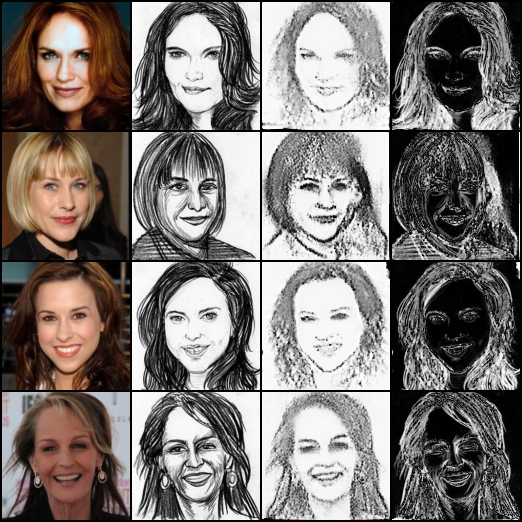
\includegraphics[width=\columnwidth]{task4/failure_cases.png}
\caption{Task 4: Failure cases with highest L1 error, typically involving complex backgrounds or unusual lighting.}
\label{fig:task4_failures}
\end{figure}

% ============================================================
\section{Comparative Analysis}
\label{sec:comparison}

\begin{table}[H]
\centering
\caption{Cross-Task Restoration Performance Comparison (N=36,690)}
\label{tab:comparison}
\begin{tabular}{lcc}
\toprule
\textbf{System} & \textbf{L1 $\downarrow$} & \textbf{SSIM $\uparrow$} \\
\midrule
Task 1: Universal AE & 0.0737 & 0.4984 \\
Task 2: Hard-Routed (predicted) & 0.0677 & 0.5370 \\
Task 3: Soft MoE & \textbf{0.0528} & \textbf{0.7029} \\
\bottomrule
\end{tabular}
\end{table}

The soft MoE demonstrates the clear advantage of differentiable, input-dependent routing over both the universal approach (28.4\% L1 improvement) and hard routing (22.0\% L1 improvement). The SSIM improvement is even more dramatic: from 0.498 (universal) to 0.703 (soft MoE), representing a 41\% increase in structural fidelity. This is attributable to the soft system's ability to blend expert outputs proportionally to corruption severity, maintaining high-frequency detail from the identity branch while leveraging specialist restoration when needed.

% ============================================================
\section{ONNX Export and Verification}
\label{sec:onnx}

All models were exported to ONNX format using \texttt{torch.onnx.export()} with dynamic batch axes:

\begin{table}[H]
\centering
\caption{ONNX Model Inventory}
\label{tab:onnx}
\begin{tabular}{lcc}
\toprule
\textbf{Model} & \textbf{File Size} & \textbf{Opset} \\
\midrule
Universal AE & 113 MB & 17 \\
Classifier & 1.0 MB & 17 \\
Specialist (S\&P) & 72.5 MB & 17 \\
Specialist (Blur) & 72.5 MB & 17 \\
Specialist (Occ) & 72.5 MB & 17 \\
Soft MoE & 218.6 MB & 14 \\
Generator & 117.3 MB & 17 \\
\bottomrule
\end{tabular}
\end{table}

Each export follows a strict verification pipeline:
\begin{enumerate}
    \item Structural validity check via \texttt{onnx.checker.check\_model()}.
    \item Numerical consistency verification by comparing PyTorch and ONNX Runtime outputs on random input tensors.
    \item All models pass with maximum absolute difference $< 10^{-5}$.
\end{enumerate}

Inference in the application uses \texttt{onnxruntime.InferenceSession} with the \texttt{CPUExecutionProvider} for cross-platform compatibility.

% ============================================================
\section{Application Architecture}
\label{sec:app}

\subsection{Design}

The application's visual design was prototyped in Google Stitch to establish the layout, color palette, component hierarchy, and responsive behavior before implementation (see Fig.~\ref{fig:stitch}).

\begin{figure}[H]
\centering
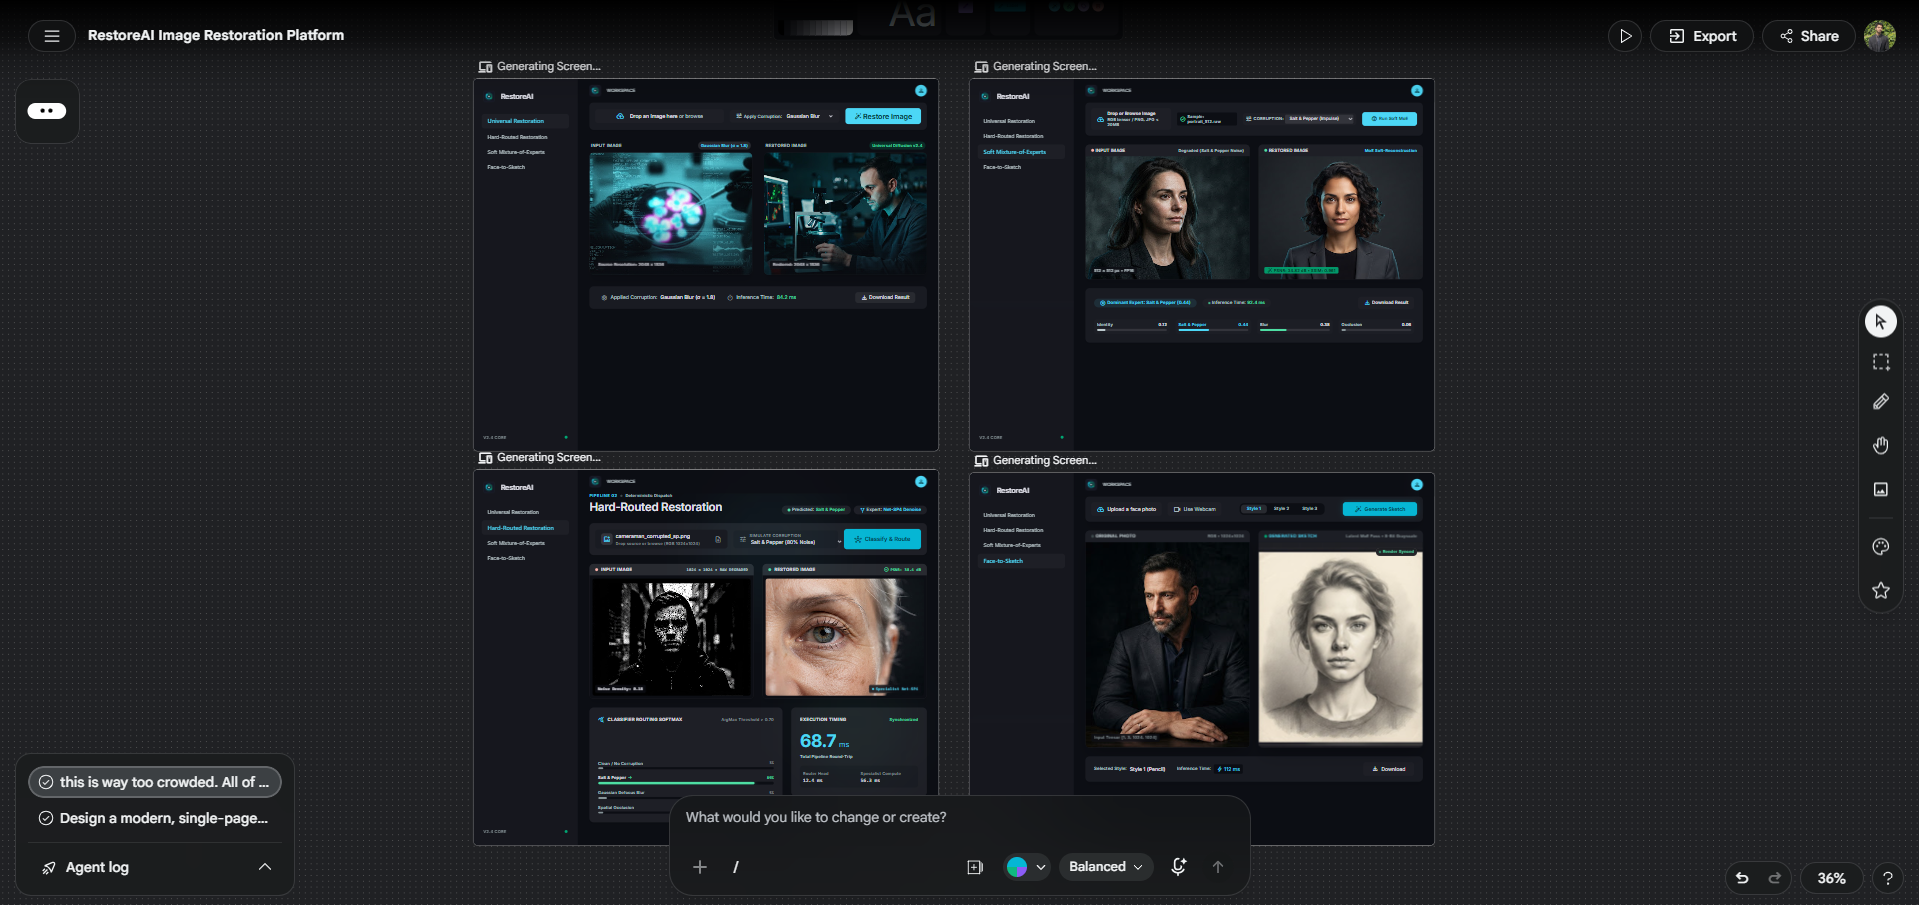
\includegraphics[width=\columnwidth]{stitch.png}
\caption{Google Stitch design prototype for the application interface.}
\label{fig:stitch}
\end{figure}

\subsection{Frontend}
The frontend is built with React and Tailwind~CSS using Vite as the build tool. It provides four workspaces accessible via a sidebar navigation. A complete 3-minute video demonstration covering all application spaces and functionalities can be viewed here: \url{https://youtu.be/CzVCmGIMKX8}.

\begin{itemize}
    \item \textbf{Universal Restoration}: Upload or select a clean image, apply corruptions via the interface, view the restored output with corruption settings and inference time.
    \item \textbf{Hard-Routed Restoration}: Displays classifier probabilities, predicted corruption, selected expert, reconstructed image, and timing breakdown.
    \item \textbf{Soft Mixture-of-Experts Restoration}: Shows all four routing weights, reconstructed result, inference time, and visual indication of dominant experts.
    \item \textbf{Face-to-Sketch Generator}: Upload a photo or capture via webcam, select Style~1/2/3, generate and download sketches.
\end{itemize}

\subsection{Backend}
The FastAPI backend provides five endpoint groups: health check, universal restoration, hard routing, soft mixture, and face-to-sketch generation. On startup, all seven ONNX models are loaded into memory via a singleton \texttt{ModelManager}. Each endpoint validates uploaded files, preprocesses images to the correct format ($128 \times 128$, NCHW, appropriate normalization), runs ONNX inference, and returns base64-encoded result images with timing information.

\subsection{Deployment}
The application is containerized with Docker Compose:
\begin{itemize}
    \item \textbf{Backend container}: Python 3.12 slim, Uvicorn server on port~8000. ONNX models are mounted as read-only volumes.
    \item \textbf{Frontend container}: Multi-stage build (Node 20 Alpine $\rightarrow$ Nginx Alpine) serving the production bundle on port~80/3000.
\end{itemize}

A single \texttt{docker-compose up --build} command starts the complete application.

% ============================================================
\section{Limitations and Future Work}
\label{sec:limitations}

\begin{enumerate}
    \item \textbf{Resolution constraint}: All models operate at $128 \times 128$. Higher-resolution restoration would require progressive architectures or patch-based processing.
    \item \textbf{Occlusion inpainting}: The strict bottleneck autoencoder fundamentally cannot hallucinate semantically plausible content for large missing regions. Diffusion-based or transformer-based inpainting would be more appropriate.
    \item \textbf{Identity dominance in Soft MoE}: The gating network over-relies on the identity branch for Gaussian blur inputs, suggesting that the blur expert's reconstruction does not sufficiently exceed the quality of the raw input. Curriculum-based training or per-expert auxiliary losses could address this.
    \item \textbf{Style imbalance in FS2K}: Style~2 has only 46 test images, making its metrics statistically less reliable. Few-shot learning or style augmentation could improve robustness.
    \item \textbf{GAN evaluation}: L1 and SSIM are imperfect metrics for generative quality. Fréchet Inception Distance (FID) would provide a more perceptually meaningful evaluation.
\end{enumerate}

% ============================================================
\section{Conclusion}
\label{sec:conclusion}

This work demonstrates a systematic progression from a monolithic universal autoencoder to a differentiable soft mixture-of-experts system, achieving a 28.4\% reduction in L1 loss and a 41\% improvement in SSIM on the Oxford-IIIT Pet corruption restoration benchmark. The corruption classifier achieves 98.26\% accuracy with per-class F1 scores exceeding 97\%, and the MoE routing analysis reveals interpretable, severity-adaptive expert allocation. The conditional GAN successfully generates style-conditioned facial sketches, with the full pipeline deployed as a single-command Dockerized web application. All models maintain ONNX numerical consistency below $10^{-5}$ tolerance, and every critical hyperparameter was systematically investigated through Optuna studies with 20 trials per task, tracked via Weights~\&~Biases.

% ============================================================
\appendices

\section{AI-Use Disclosure}
\label{appendix:ai}

The following AI tools were used during the development of this project:

\begin{itemize}
    \item \textbf{Google Antigravity (Gemini-based coding assistant)}: Used for code scaffolding, debugging, architecture prototyping, and report drafting. All generated code was manually verified, tested with custom unit tests, and modified to meet specific assignment requirements. Training scripts, evaluation pipelines, and ONNX exports were validated end-to-end before inclusion.
    \item \textbf{Google Stitch}: Used for UI/UX design prototyping of the application interface.
    \item \textbf{Weights \& Biases}: Used for automated experiment tracking, loss curve visualization, and hyperparameter comparison across Optuna trials.
\end{itemize}

All AI-generated outputs were critically evaluated, tested against expected behavior, and corrected where necessary. The student maintains full understanding of every component in the submitted system.

% ============================================================
% References
% ============================================================
\begin{thebibliography}{00}

\bibitem{zhang2017beyond}
K.~Zhang, W.~Zuo, Y.~Chen, D.~Meng, and L.~Zhang, ``Beyond a Gaussian denoiser: Residual learning of deep CNN for image denoising,'' \textit{IEEE Trans. Image Process.}, vol.~26, no.~7, pp.~3142--3155, 2017.

\bibitem{vincent2008extracting}
P.~Vincent, H.~Larochelle, Y.~Bengio, and P.~A.~Manzagol, ``Extracting and composing robust features with denoising autoencoders,'' in \textit{Proc. ICML}, 2008, pp.~1096--1103.

\bibitem{mao2016image}
X.~Mao, C.~Shen, and Y.~Yang, ``Image restoration using very deep convolutional encoder-decoder networks with symmetric skip connections,'' in \textit{Proc. NIPS}, 2016, pp.~2802--2810.

\bibitem{jacobs1991adaptive}
R.~A.~Jacobs, M.~I.~Jordan, S.~J.~Nowlan, and G.~E.~Hinton, ``Adaptive mixtures of local experts,'' \textit{Neural Comput.}, vol.~3, no.~1, pp.~79--87, 1991.

\bibitem{shazeer2017outrageously}
N.~Shazeer, A.~Mirzadeh, K.~Maziarz, A.~Davis, Q.~Le, G.~Hinton, and J.~Dean, ``Outrageously large neural networks: The sparsely-gated mixture-of-experts layer,'' in \textit{Proc. ICLR}, 2017.

\bibitem{fedus2022switch}
W.~Fedus, B.~Zoph, and N.~Shazeer, ``Switch transformers: Scaling to trillion parameter models with simple and efficient sparsity,'' \textit{J. Mach. Learn. Res.}, vol.~23, no.~120, pp.~1--39, 2022.

\bibitem{isola2017image}
P.~Isola, J.-Y.~Zhu, T.~Zhou, and A.~A.~Efros, ``Image-to-image translation with conditional adversarial networks,'' in \textit{Proc. CVPR}, 2017, pp.~1125--1134.

\bibitem{fan2022facial}
Y.~Fan, L.~Liu, F.~Chen, Y.~Luo, and K.~Zhang, ``FS2K: A facial sketch synthesis dataset,'' in \textit{Proc. AAAI}, 2022.

\bibitem{wang2004image}
Z.~Wang, A.~C.~Bovik, H.~R.~Sheikh, and E.~P.~Simoncelli, ``Image quality assessment: From error visibility to structural similarity,'' \textit{IEEE Trans. Image Process.}, vol.~13, no.~4, pp.~600--612, 2004.

\bibitem{ioffe2015batch}
S.~Ioffe and C.~Szegedy, ``Batch normalization: Accelerating deep network training by reducing internal covariate shift,'' in \textit{Proc. ICML}, 2015, pp.~448--456.

\bibitem{odena2016deconvolution}
A.~Odena, V.~Dumoulin, and C.~Olson, ``Deconvolution and checkerboard artifacts,'' \textit{Distill}, 2016.

\end{thebibliography}

\end{document}
